\documentclass[12pt, a4paper]{report}
\setlength{\headheight}{14.5pt}
\usepackage{thesis} % Ensure thesis.sty exists or remove if unnecessary

% Include necessary libraries

\setlength{\tabcolsep}{4pt}
\usepackage{longtable}
\usepackage{booktabs}
\usepackage{array}
\usepackage{caption}
\newcolumntype{L}[1]{>{\raggedright\arraybackslash}p{#1}}

\usepackage{pdflscape}
\usepackage{array}
\usepackage{graphicx}
\usepackage{float}
\usepackage{graphicx}
\usepackage{float}
\usepackage{titling}
\usepackage{comment}
\usepackage{subfig}
\usepackage{lipsum}
\usepackage[tableposition=top]{caption}
\usepackage[Glenn]{fncychap}
\usepackage{hyperref}
\hypersetup{
    citecolor=blue,
    urlcolor=blue,
}

% Custom commands
\newcommand{\dept}{Computer Science and Engineering}
\newcommand{\department}{Department of Computer Science and Engineering}
\newcommand{\university}{Premier University, Chittagong}

\newcommand{\chairmanName}{Dr. Shahid Md. Asif Iqbal}
\newcommand{\chairmanDesignation}{Professor and Chairman}

\newcommand{\supervisorName}{Avisheak Das}
\newcommand{\supervisorDesignation}{Lecturer}

% Update with actual author names and IDs
\newcommand{\firstAuthorName}{Mohammad Hafizur Rahman Sakib}
\newcommand{\firstAuthorId}{0222210005101118}
\newcommand{\secondAuthorName}{Arnab Shikder}
\newcommand{\secondAuthorId}{0222210005101098}
\newcommand{\thirdAuthorName}{Mohammad Asmual Hoque Yousha}
\newcommand{\thirdAuthorId}{0222210005101121}

\newcommand{\projectTitle}{LeafGuard: Deep Learning-Based Detection of Cassava Plant Diseases}

\begin{document}

\pagenumbering{roman}
\renewcommand{\contentsname}{Table of Contents}
\tableofcontents

\clearpage
\addcontentsline{toc}{chapter}{List of Figures}
\listoffigures

\clearpage
\addcontentsline{toc}{chapter}{List of Tables}
\listoftables
% Abstract
\clearpage
\thispagestyle{plain}
\begin{center}
    \LARGE{\textbf{Abstract}}
\end{center}
The “Odyssey Travel Agency Software” is a full-stack web application designed to simplify and enhance the travel booking process for users and administrators alike. Users can register, browse country-specific tour packages, select desired packages, choose flight and hotel preferences, and proceed to book through a secure payment gateway. The frontend leverages HTML, CSS, Tailwind CSS, JavaScript, and Next.js for a responsive and interactive user experience, while the backend is powered by Laravel and MySQL for efficient data processing and management. The admin interface allows CRUD operations on tour packages and facilitates the addition of local tour guide details. The system is developed following core software engineering principles such as modularity, scalability, and user-centric design, ensuring the product is both robust and maintainable for long-term use.

\textbf{Keywords:} Travel Booking System, Laravel, Next.js, Tour Packages, Full-Stack Web Application, Payment Gateway, Admin Panel, CRUD Operations

\vspace{0.5cm}

\noindent GitHub Repository:
\href{https://github.com/ArnabShikder24/odyssey-travel-client}{\textbf{https://github.com/ArnabShikder24/odyssey-travel-client}} 



% Switch to arabic numbering for main chapters
\clearpage
\pagenumbering{arabic}
\setcounter{page}{1}

% Chapters
\clearpage
\chapter{Introduction}
\section{Background}
Cassava is a staple food crop grown in tropical and subtropical regions. It is valued for its high-yield tubers and nutrient-rich leaves. Its resilience in poor soils makes it a vital food source in many low-income regions. However, cassava plants are highly susceptible to several leaf diseases including Cassava Bacterial Blight (CBB), Cassava Brown Streak Disease (CBSD), Cassava Green Mottle (CGM), and Cassava Mosaic Disease (CMD). These diseases disrupt the photosynthetic process and significantly reduce crop yield and quality.

Conventional methods of disease detection involve laboratory testing or expert consultation, both of which are costly and time-consuming. As a result, farmers often lack the means to detect and treat diseases early. With recent advances in machine learning, especially in image classification using deep learning, it is now possible to build systems that can classify crop diseases from images with high accuracy and low cost. This project applies such techniques to develop a cassava leaf disease detection system.

\section{Problem Statement}
In regions like Bangladesh, where cassava is not yet widely cultivated but has strong potential, there is limited infrastructure for disease monitoring. Farmers lack tools for early and accurate identification of leaf diseases. Manual diagnosis is often not viable due to lack of expertise, cost, and time constraints.

This research focuses on the classification of cassava leaf diseases using machine learning models trained on labeled image datasets. The goal is to evaluate various deep learning models to determine which provides the best trade-off between accuracy and computational efficiency, ultimately aiding in timely and scalable disease detection.

\section{Chapter Distribution}
This report is organized into the following chapters:

\begin{itemize}
    \item \textbf{Chapter 1: Introduction} — Introduces the background of the study, identifies the research problem, and outlines the structure of the report.
    
    \item \textbf{Chapter 2: Literature Review} — Summarizes related works from at least eight research papers relevant to crop disease classification, focusing on methods, datasets, and performance metrics.

    \item \textbf{Chapter 3: Methodology} — Describes the overall method used in the project, details the machine learning models implemented, and explains the proposed framework that yielded the best performance.

    \item \textbf{Chapter 4: Experimental Result and Analysis} — Provides a description of the dataset, evaluation metrics, and parameter settings. It also discusses experimental results in detail, including error analysis, limitations, and the social or cultural impact of the proposed solution.

    \item \textbf{Chapter 5: Conclusion and Future Work} — Summarizes the research findings, reflects on the limitations, and suggests directions for future improvements and further study.
\end{itemize}



\clearpage
\chapter{Literature Review} \label{ch: reviews}
\section{Introduction}
Plant diseases continue to pose a significant threat to global food security, particularly in regions heavily reliant on agriculture. Among various crops, cassava is a crucial staple in many developing countries, making the early detection of its diseases a priority. This section introduces the importance of automated plant disease detection systems and the motivation behind leveraging deep learning techniques, especially convolutional neural networks (CNNs), for this purpose. Our project, LeafGuard, builds on this foundation to detect cassava diseases using image-based analysis.

\section{Background Study}
Traditional methods for plant disease detection, such as expert consultation and laboratory testing, are often time-consuming, costly, and inaccessible to small-scale farmers. The evolution of machine learning and, more recently, deep learning, has opened new possibilities in automating disease detection from leaf images.

Numerous studies have shown the effectiveness of CNNs in classifying plant diseases. For example, researchers like Ramcharan et al. (2017) have developed mobile-based applications for cassava disease detection with high accuracy using deep learning. Public datasets such as PlantVillage and custom datasets of cassava leaf images have facilitated significant progress in this area. Data augmentation techniques, including rotation, flipping, and contrast adjustments, are commonly applied to increase dataset diversity and improve model generalization.

Challenges still remain, including varying lighting conditions, background noise, and differences in leaf appearance due to age or environmental factors. These are important considerations addressed in our methodology and system design.

\subsection{Software Design Pattern}
For the software architecture of LeafGuard, we adopted the Model-View-Controller (MVC) design pattern. This design approach enhances code organization and allows for independent development, testing, and scaling of components.

\begin{itemize}
    \item \textbf{Model:} Manages data-related logic, such as loading the trained CNN model, preprocessing input images, and outputting predictions.
    \item \textbf{View:} Responsible for the user interface, where users can upload leaf images and view the classification results.
    \item \textbf{Controller:} Acts as a bridge between the view and model, processing user inputs, invoking the model, and updating the interface with predictions.
\end{itemize}

The MVC pattern allows us to decouple the logic of disease detection from the presentation layer. This modularity is particularly useful when upgrading the model or expanding the user interface in future versions.

\section{Summary}
This chapter reviewed the foundational work and research relevant to plant disease detection using image classification. The rapid advancement of deep learning, especially CNNs, has made high-accuracy leaf disease detection feasible. Coupled with a modular design approach such as MVC, our project aims to deliver a robust, user-friendly, and scalable solution for cassava disease detection. The insights gained here inform the methodology used in our implementation, which is detailed in the following chapter.


\clearpage
\chapter{Methodology} \label{ch: methodology}
\section{Methodology}
This section outlines the systematic approach followed during the development of the travel agency website. The Software Development Life Cycle (SDLC) model was followed to ensure that the project was well-organized, efficient, and delivered successfully within the given timeframe.

\subsection{Planning}
The planning phase involved identifying project goals, features, and tools. The stack was finalized to include HTML, Tailwind CSS, JavaScript, and Next.js for the frontend, and Laravel with MySQL for the backend. Requirements were gathered for both the user and admin roles, and the expected user journey was mapped out—from viewing packages to payment completion.

\subsection{Design}
The design phase included both frontend and backend architectural planning. Wireframes were drawn to visualize page layouts such as Home, Package Listing, and Booking pages. The backend was structured using Laravel's MVC architecture. ER diagrams were created to model database relationships for users, packages, bookings, and tour guides.

\subsection{Implementation}
Frontend pages were built using Next.js for server-side rendering and faster load times. Tailwind CSS was used for consistent, responsive styling. On the backend, Laravel handled routing, controllers, models, and database migrations. Admin features like CRUD operations for tour packages and guide management were also implemented here.

\subsection{Testing}
Unit and integration testing were carried out to ensure all features worked as intended. Laravel’s built-in testing tools were used to test backend logic. Frontend behavior was manually tested across different browsers and devices. Form validation and session handling were thoroughly checked.

\subsection{Deployment}
After successful testing, the application was prepared for deployment. The backend (Laravel) was hosted on a PHP-compatible server, and the Next.js frontend was deployed via Vercel or a Node-compatible server. Environment variables were configured for secure communication with the database and third-party services.

\subsection{Future Enhancements}
Possible future improvements include integrating a real-time chatbot for customer support, adding review and rating features for packages, incorporating real-time availability for flights and hotels via APIs, and building a mobile app version of the platform using React Native.


\clearpage
\chapter{Diagram} \label{ch: diagram}
\section{Diagrams}

\subsection{UML (Unified Modeling Language)}
UML (Unified Modeling Language) is a standardized modeling language used to visualize, design, and document the structure and behavior of software systems. It provides a graphical representation of the system architecture, relationships, and interactions between components.

\vspace{0.5cm}
\begin{center}
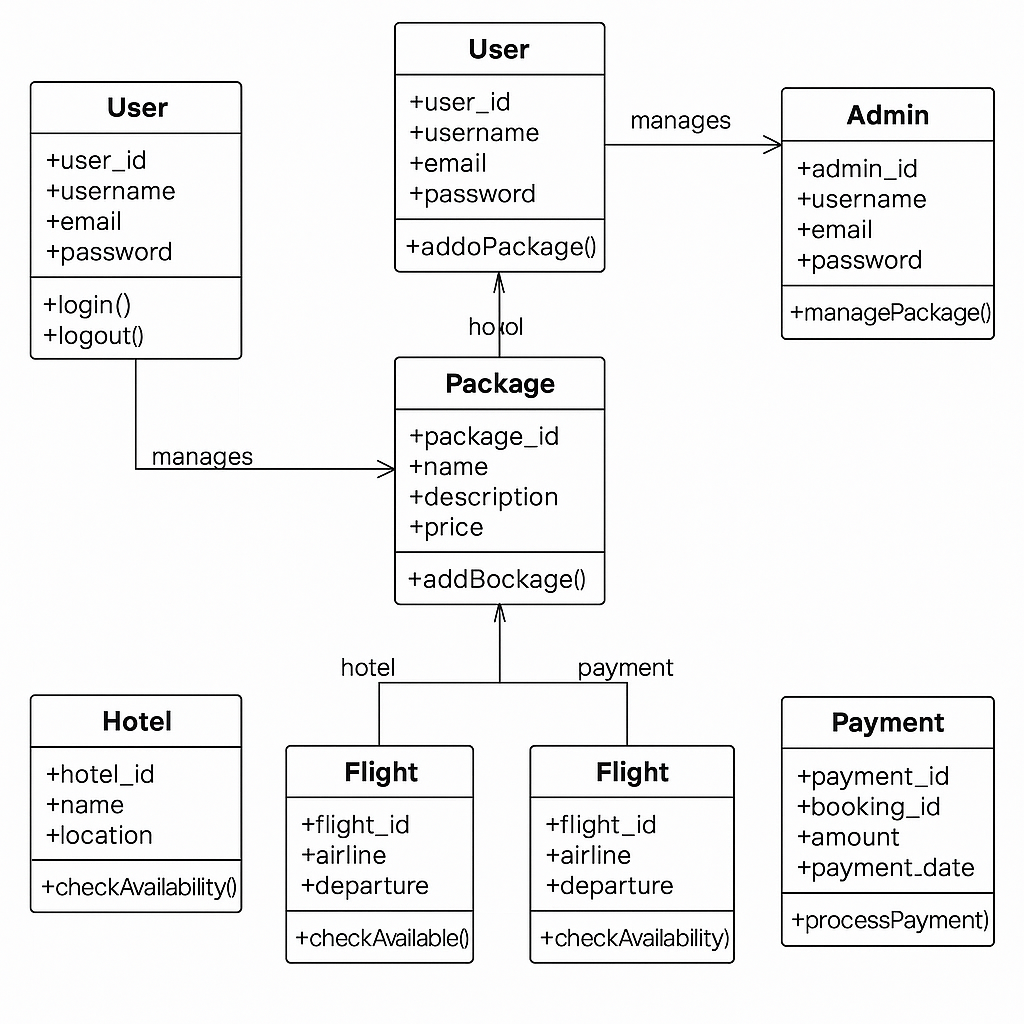
\includegraphics[width=1.0\textwidth]{./figures/UML Diagram/uml2.0.png} % Replace with your actual UML diagram path
\captionof{figure}{UML Diagram}
\end{center}
\vspace{0.5cm}

\subsection{Activity Diagram}
\subsubsection{Description}
An Activity Diagram models the flow of control in a system, representing the sequence of activities and their transitions. It visually represents workflows such as business processes or the flow of an algorithm, using actions, decisions, start and end points, and parallel processing.

\subsubsection{Usage}
\begin{itemize}
    \item \textbf{Workflow Representation:} Used to model high-level business processes or system workflows.
    \item \textbf{Decision Making:} Helps in visualizing conditional logic, showing decision points and alternative flows.
    \item \textbf{Parallel Processes:} Represents parallel processing or branching in a system.
\end{itemize}

\subsubsection{Key Elements}
\begin{itemize}
    \item \textbf{Initial Node:} Marks the starting point of the process.
    \item \textbf{Activity/Action:} Represents tasks or operations performed.
    \item \textbf{Decision Node:} Represents branching in the workflow, where a choice must be made.
    \item \textbf{Merge Node:} Combines multiple flows back into a single flow after decision points.
    \item \textbf{Final Node:} Marks the end of the process.
\end{itemize}

\vspace{0.5cm}
\begin{center}
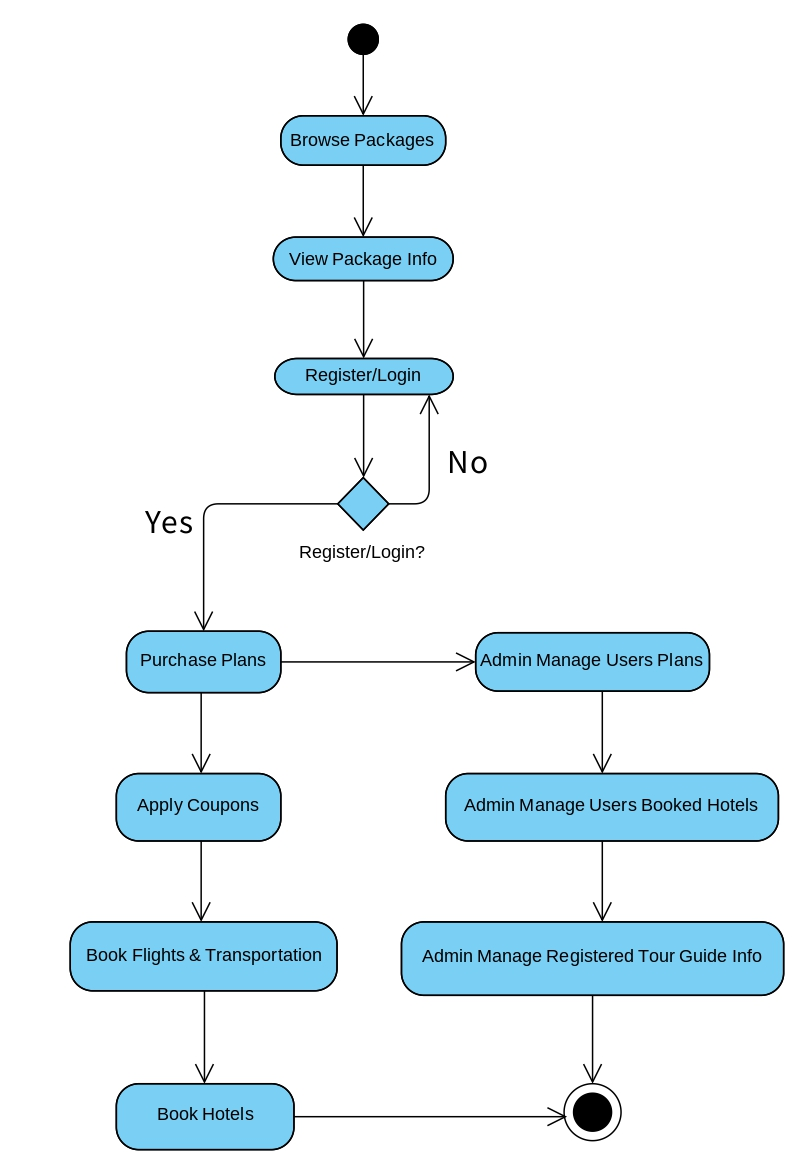
\includegraphics[width=1.0\textwidth]{./figures/Activity Diagram/actd.jpg} % Replace with your actual Activity Diagram path
\captionof{figure}{Activity Diagram for Odyssey Travel Agency Software}
\end{center}
\vspace{0.5cm}


\vspace{0.5cm}
\begin{center}
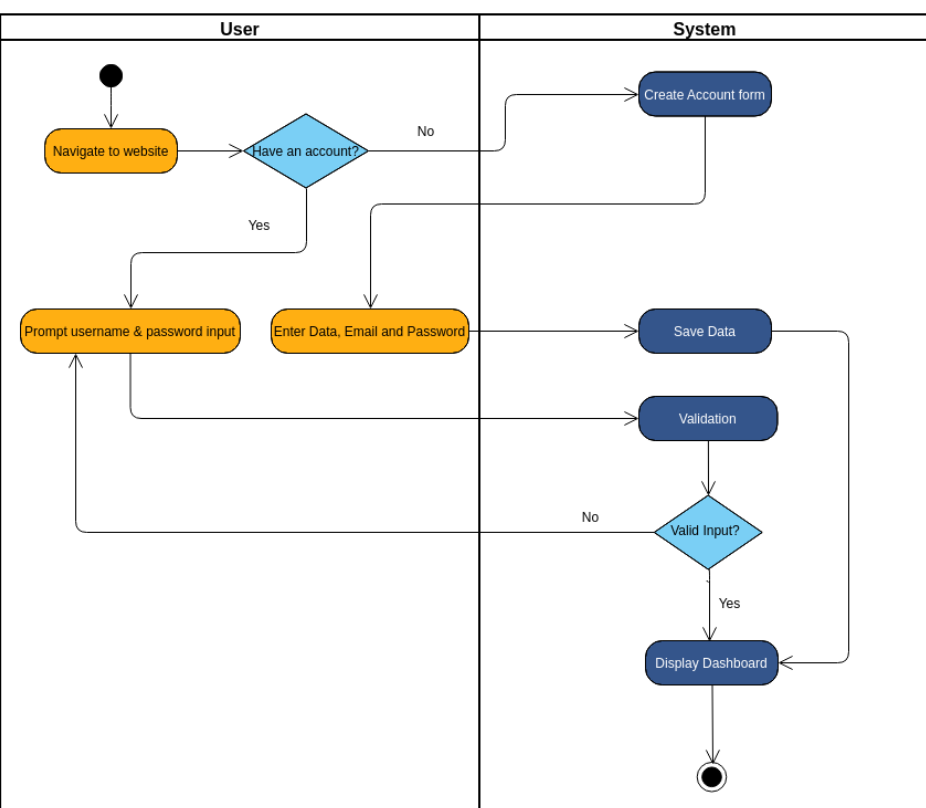
\includegraphics[width=0.8\textwidth]{./figures/Activity Diagram/1_reg.png} % Replace with your actual Activity Diagram path
\captionof{figure}{Activity Diagram Of Login and Registra   tion System} 
\end{center}
\vspace{0.5cm}

\vspace{0.5cm}
\begin{center}
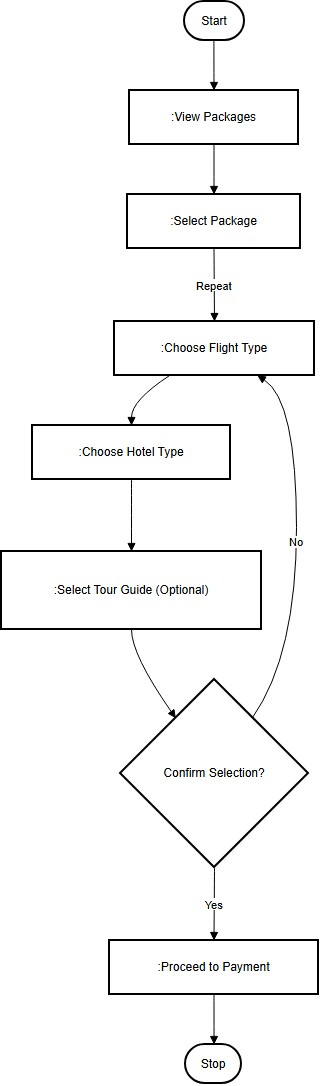
\includegraphics[width=0.5\textwidth]{./figures/Activity Diagram/2_activity.jpg} % Replace with your actual Activity Diagram path
\captionof{figure}{Package Selection Activity Diagram}
\end{center}
\vspace{0.5cm}

\vspace{0.5cm}
\begin{center}
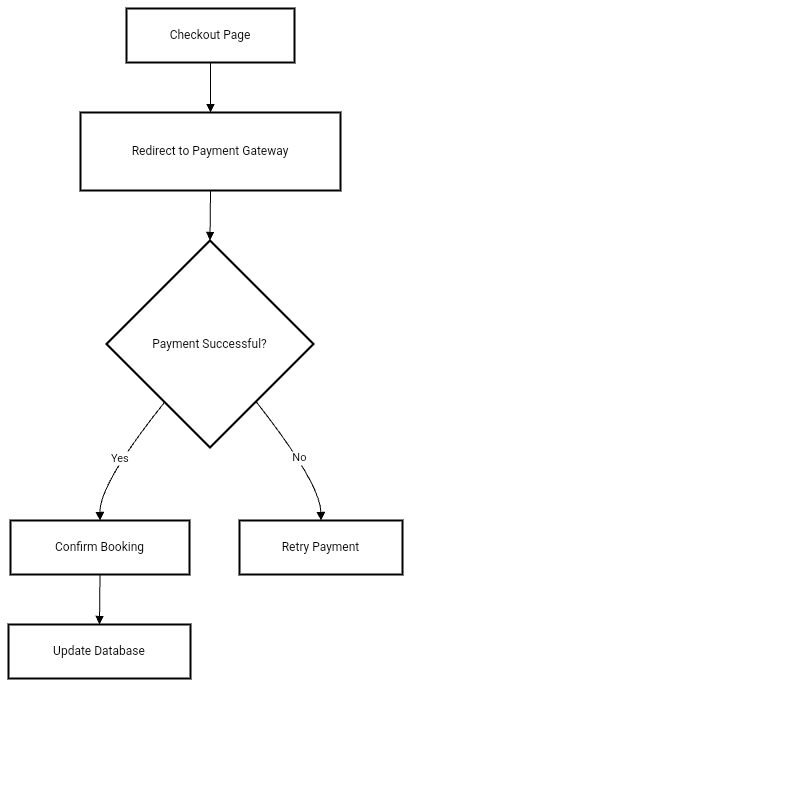
\includegraphics[width=0.8\textwidth]{./figures/Activity Diagram/3_acivity.png} % Replace with your actual Activity Diagram path
\captionof{figure}{Payment System Activity Diagram}
\end{center}
\vspace{0.5cm}

\vspace{0.5cm}
\begin{center}
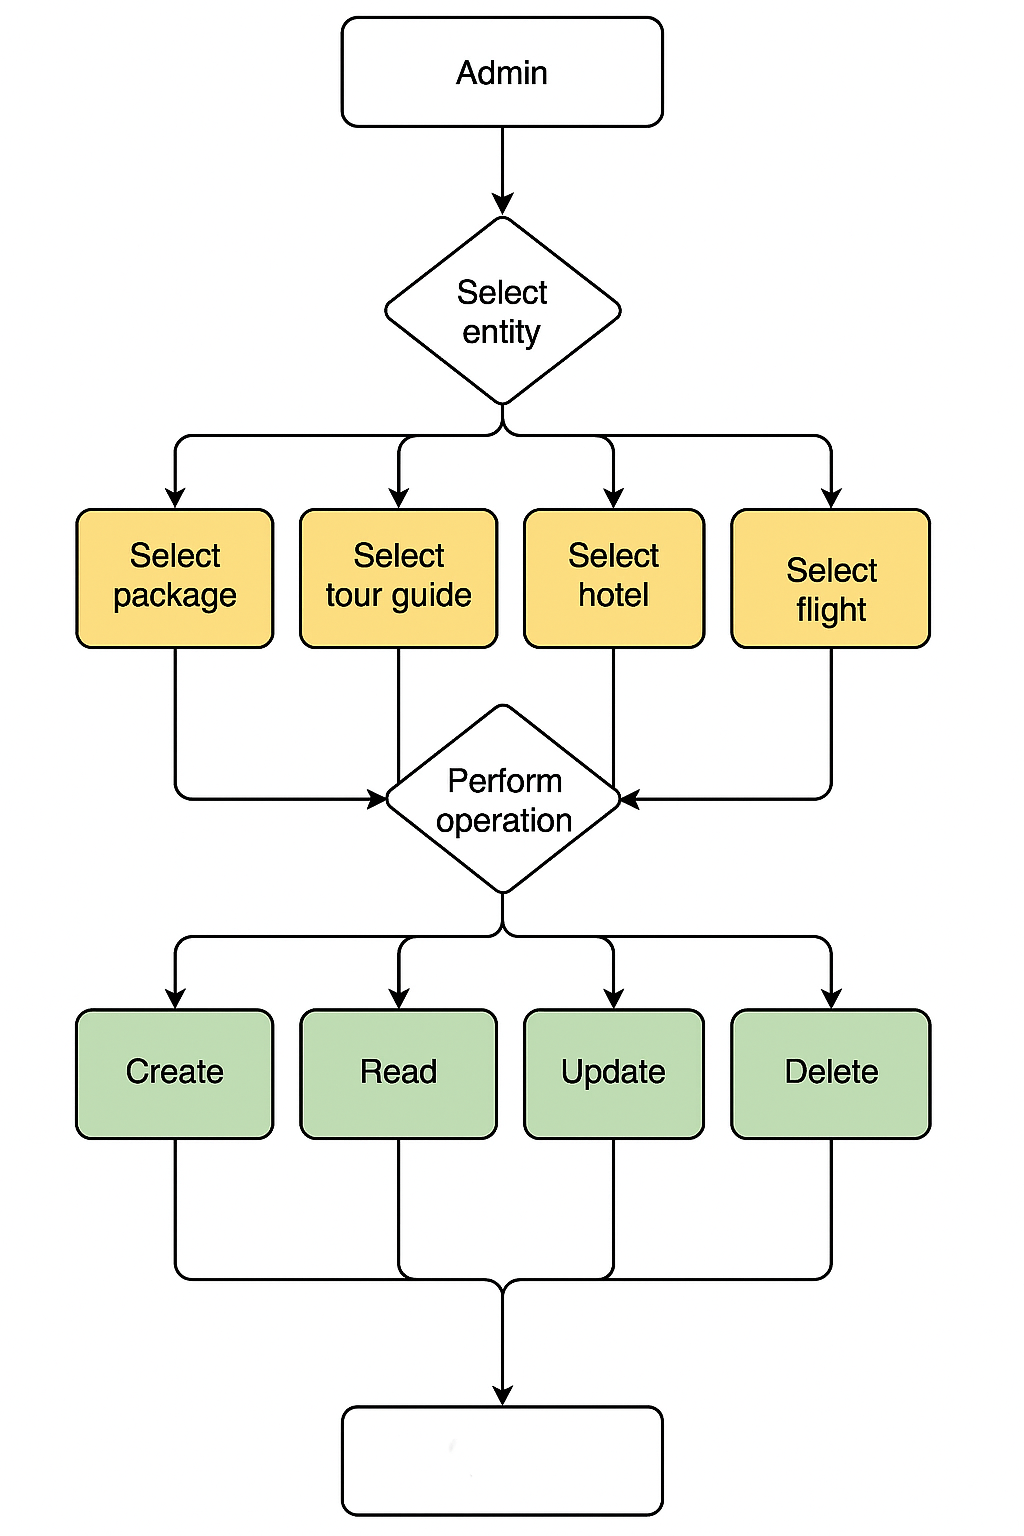
\includegraphics[width=0.8\textwidth]{./figures/Activity Diagram/4_crud_activity.png} % Replace with your actual Activity Diagram path
\captionof{figure}{Admin CRUD Operation Activity Diagram}
\end{center}
\vspace{0.5cm}


\subsection{Sequence Diagram}
\subsubsection{Description}
A Sequence Diagram focuses on the interaction between objects or components in a system over time. It shows the sequence of messages exchanged between objects to achieve a specific goal or functionality. It highlights the order of interactions and the roles of different components in a system.

\subsubsection{Usage}
\begin{itemize}
    \item \textbf{Object Interaction:} Helps in understanding the detailed interactions between different objects in a system.
    \item \textbf{Method Call Flow:} Useful for describing the flow of control during method calls and responses.
    \item \textbf{Debugging \& Testing:} Provides insight into the communication between objects, useful for debugging and designing test cases.
\end{itemize}

\subsubsection{Key Elements}
\begin{itemize}
    \item \textbf{Objects/Actors:} Represent entities that participate in the interaction.
    \item \textbf{Lifeline:} A dashed line that represents the lifespan of an object during the interaction.
    \item \textbf{Message Arrows:} Represent the messages sent between objects, showing the direction and order.
    \item \textbf{Activation Bar:} Indicates when an object is active (processing).
    \item \textbf{Return Message:} Represents the return of control from a method.
\end{itemize}

\vspace{0.5cm}
\begin{center}
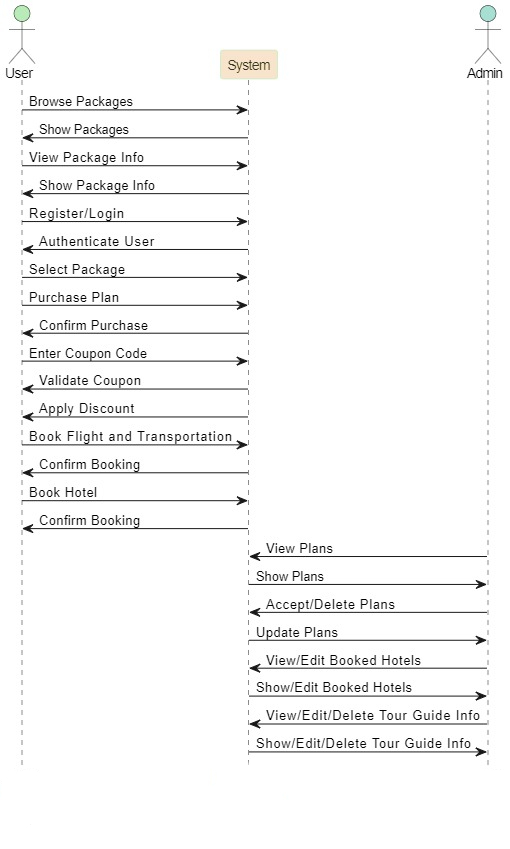
\includegraphics[width=0.8\textwidth]{./figures/Sequence Diagram/sqd.jpg} % Replace with your actual Sequence Diagram path
\captionof{figure}{Sequence Diagram of Odyssey Travel Agency Software}
\end{center}
\vspace{0.5cm}

\vspace{0.5cm}
\begin{center}
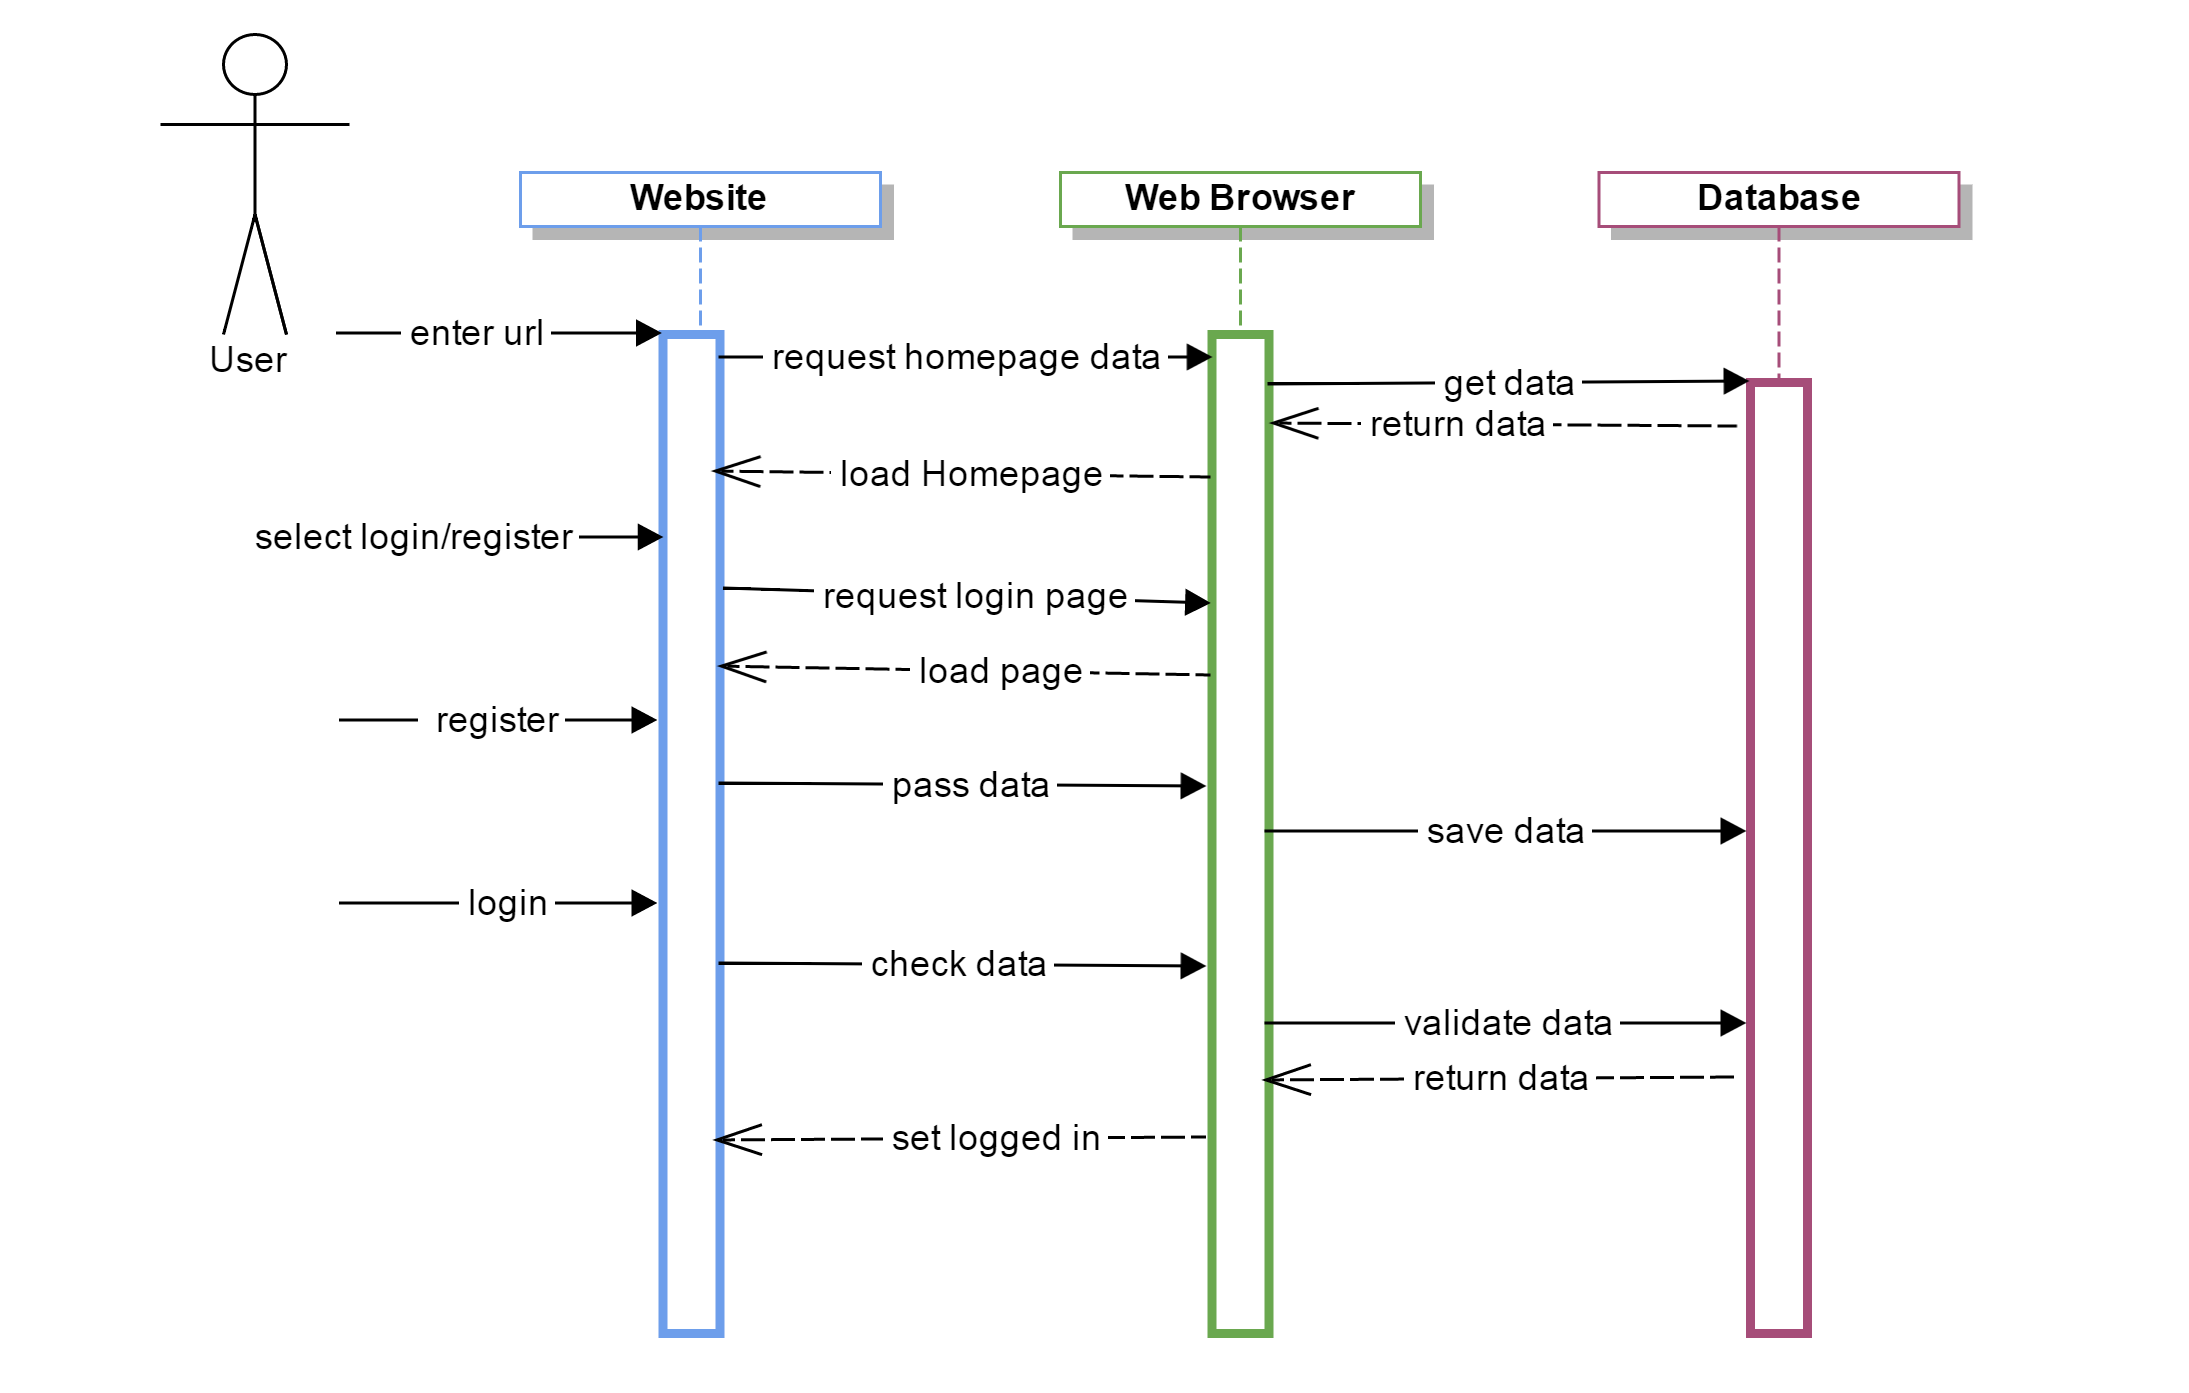
\includegraphics[width=0.9\textwidth]{./figures/Sequence Diagram/1_seq.png} % Replace with your actual Activity Diagram path
\captionof{figure}{Sequence Diagram Of Login and Registra   tion System} 
\end{center}
\vspace{0.5cm}

\vspace{0.5cm}
\begin{center}
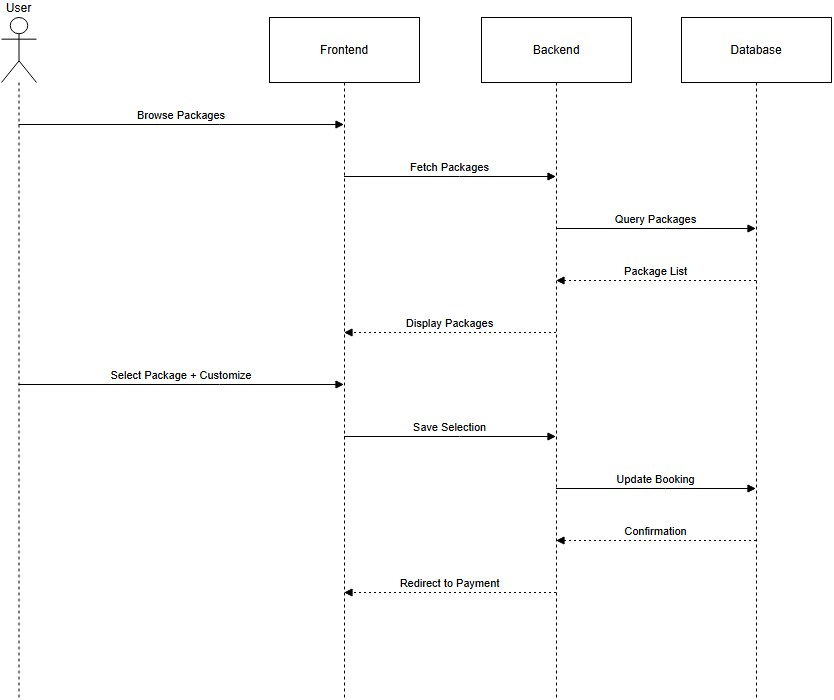
\includegraphics[width=1.0\textwidth]{./figures/Sequence Diagram/2_seq.jpg} % Replace with your actual Activity Diagram path
\captionof{figure}{Package Selection Sequence Diagram}
\end{center}
\vspace{0.5cm}

\vspace{0.5cm}
\begin{center}
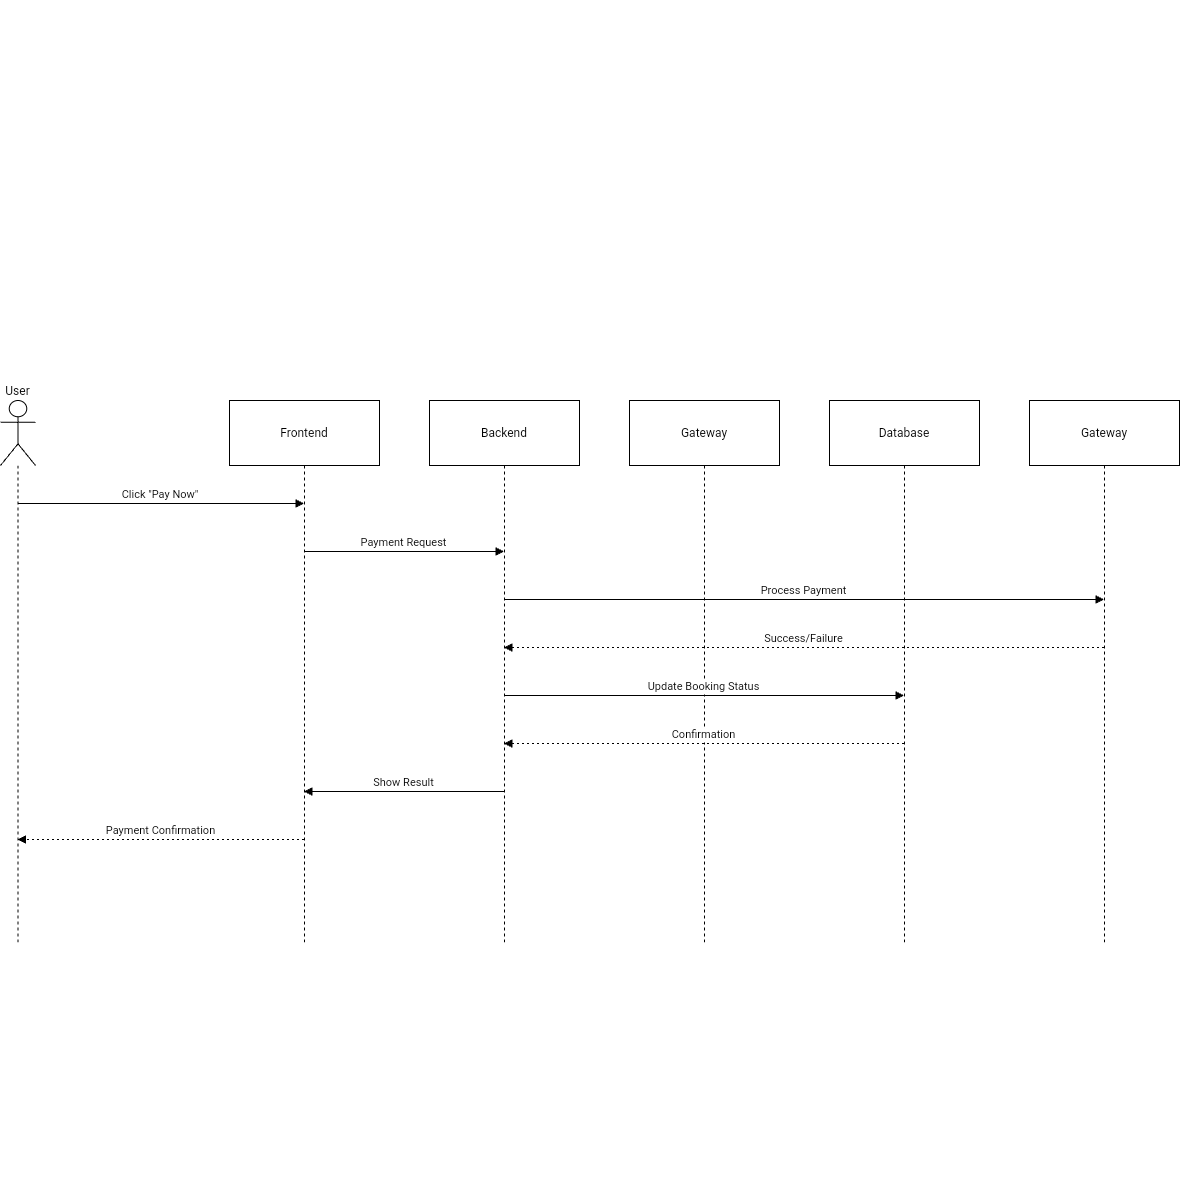
\includegraphics[width=1.0\textwidth]{./figures/Sequence Diagram/3_seq.png} % Replace with your actual Activity Diagram path
\captionof{figure}{Payment System Sequence Diagram}
\end{center}
\vspace{0.5cm}

\vspace{0.5cm}
\begin{center}
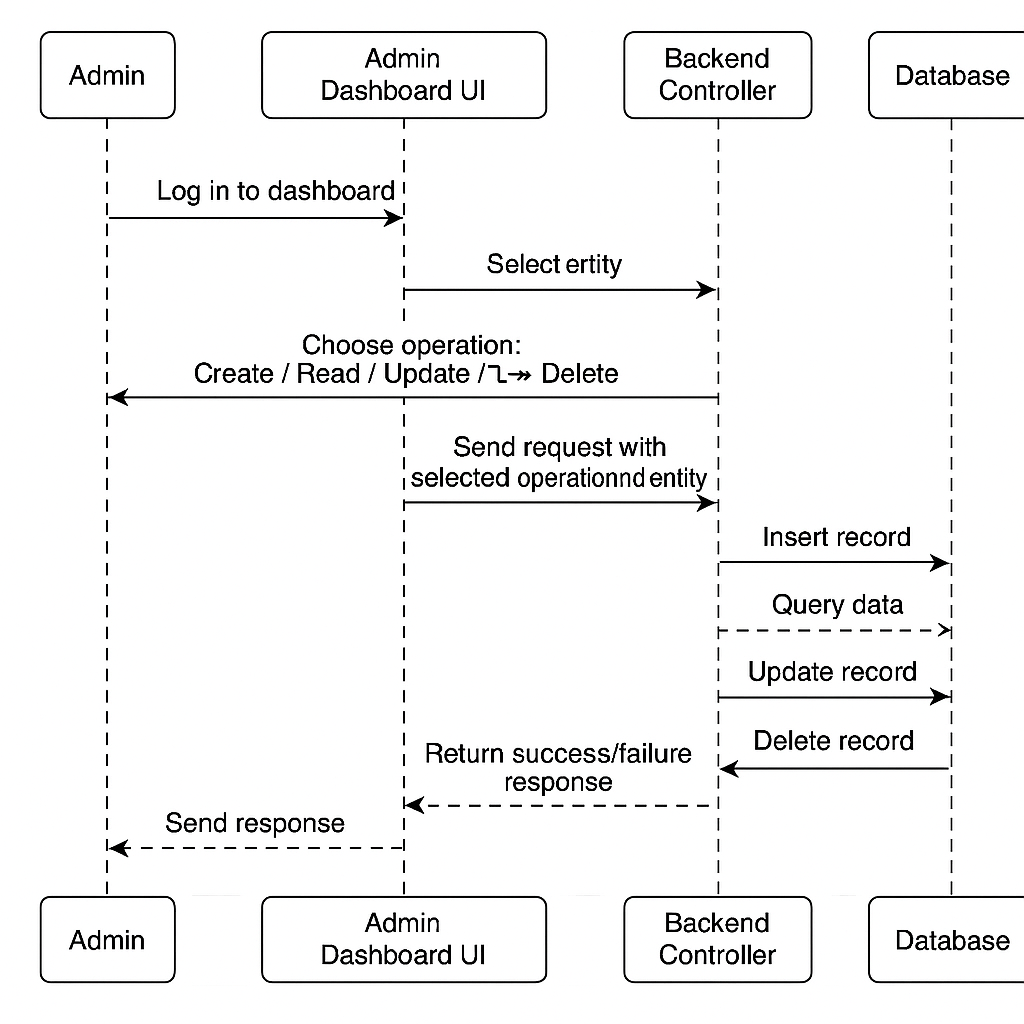
\includegraphics[width=0.8\textwidth]{./figures/Sequence Diagram/4_crud_sequence.png} % Replace with your actual Activity Diagram path
\captionof{figure}{Admin CRUD Operation Sequence Diagram}
\end{center}
\vspace{0.5cm}

\subsection{Use Case Diagram}
\subsubsection{Description}
A Use Case Diagram represents the functional requirements of a system by showing interactions between users (actors) and the system itself. It highlights the different use cases (functions or processes) the system performs and which actors are involved in each use case.

\subsubsection{Usage}
\begin{itemize}
    \item \textbf{Requirement Gathering:} Used to capture and clarify system functionality from the user's perspective.
    \item \textbf{System Scope:} Defines the boundaries of the system and what will be included in its functionality.
    \item \textbf{User Interaction:} Visualizes user-system interactions to understand how different users (actors) use the system.
\end{itemize}

\subsubsection{Key Elements}
\begin{itemize}
    \item \textbf{Actors:} Represent users or other systems that interact with the system.
    \item \textbf{Use Cases:} Represent functions or actions that the system performs (e.g., "Login," "Add Package").
    \item \textbf{System Boundary:} Represents the scope of the system and distinguishes between internal functions and external actors.
    \item \textbf{Associations:} Arrows or lines connecting actors to use cases, indicating their involvement.
\end{itemize}

\vspace{0.5cm}
\begin{center}
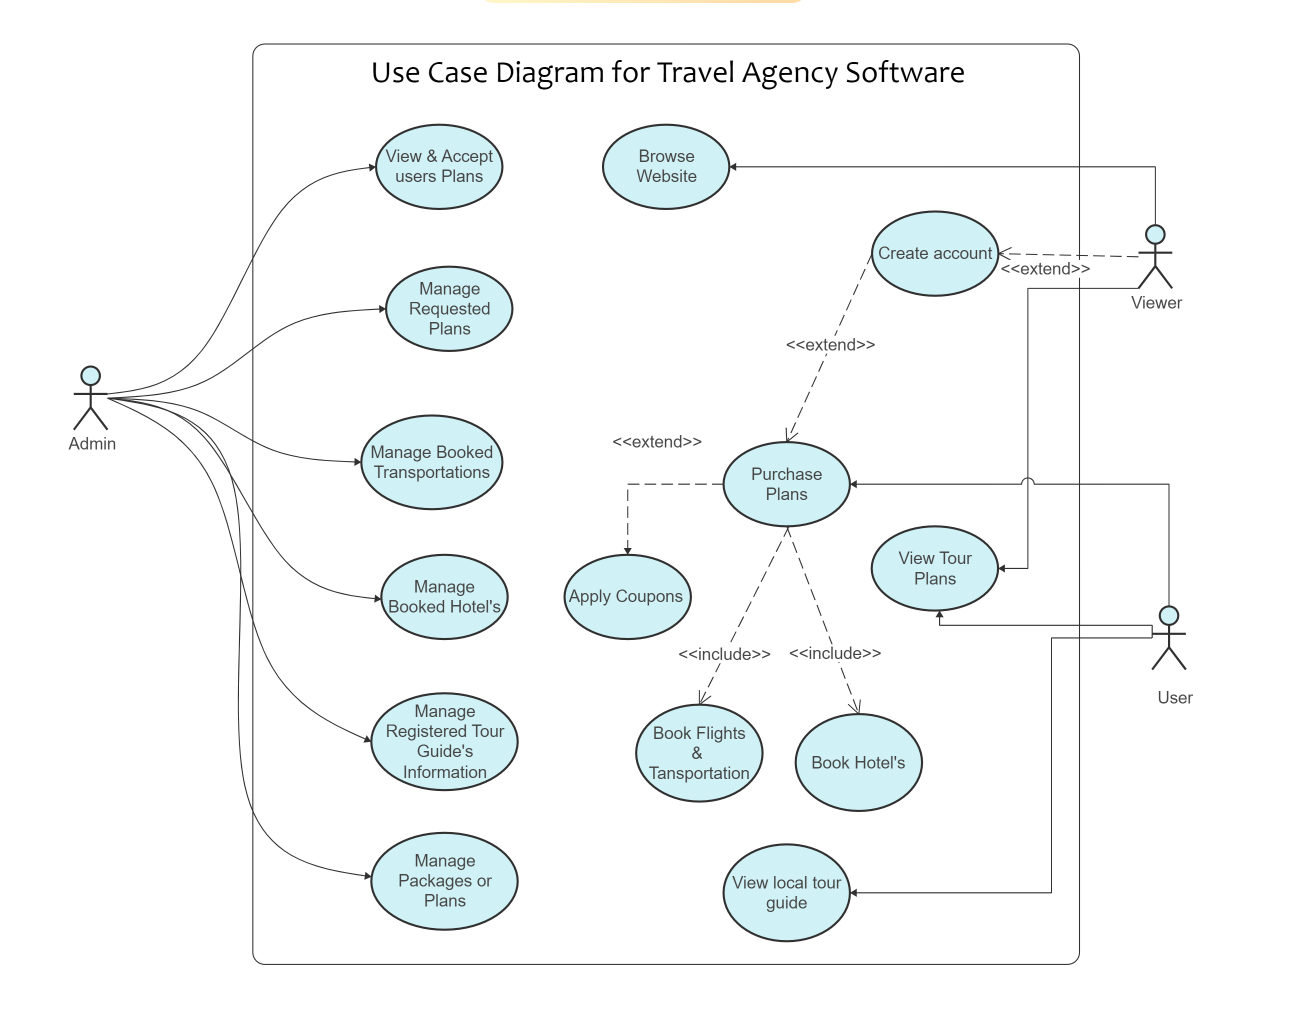
\includegraphics[width=0.8\textwidth]{./figures/Use Case Diagrams/uc_1.3.png} % Replace with your actual Use Case Diagram path
\captionof{figure}{Use Case Diagram for Odyssey Travel Agency Software}
\end{center}
\vspace{0.5cm}

\vspace{0.5cm}
\begin{center}
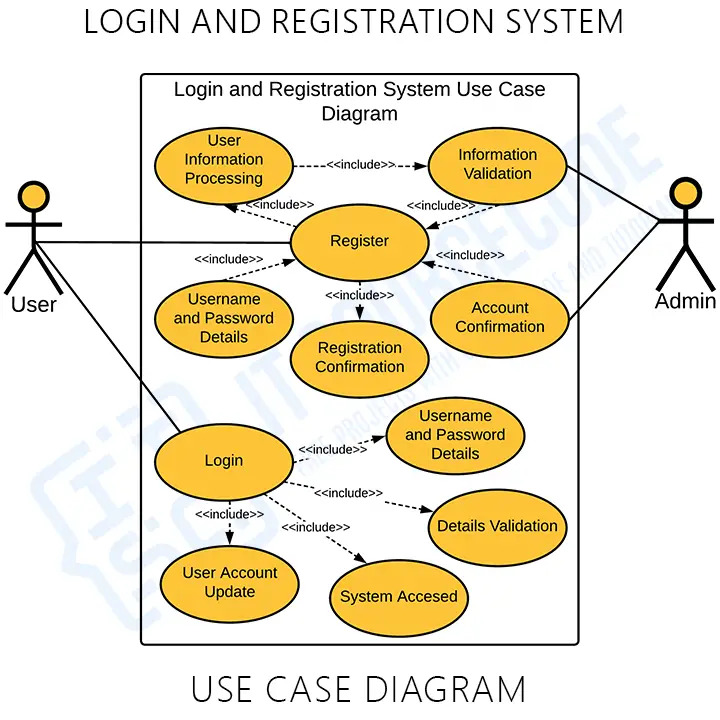
\includegraphics[width=0.8\textwidth]{./figures/Use Case Diagrams/1_usecase.jpg} % Replace with your actual Activity Diagram path
\captionof{figure}{Use Case Diagram Of Login and Registra   tion System} 
\end{center}
\vspace{0.5cm}

\vspace{0.5cm}
\begin{center}
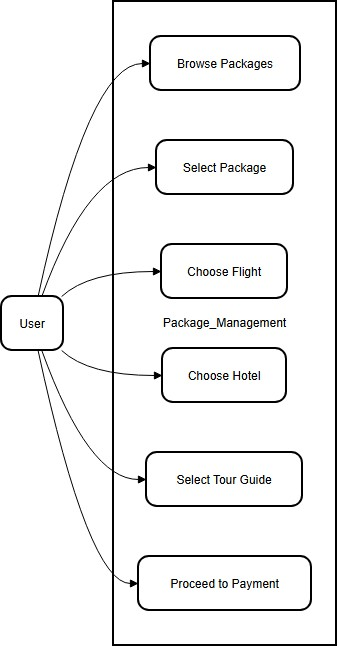
\includegraphics[width=0.5\textwidth]{./figures/Use Case Diagrams/2_usecaase.jpg} % Replace with your actual Activity Diagram path
\captionof{figure}{Package Selection Use Case Diagram}
\end{center}
\vspace{0.5cm}

\vspace{0.5cm}
\begin{center}
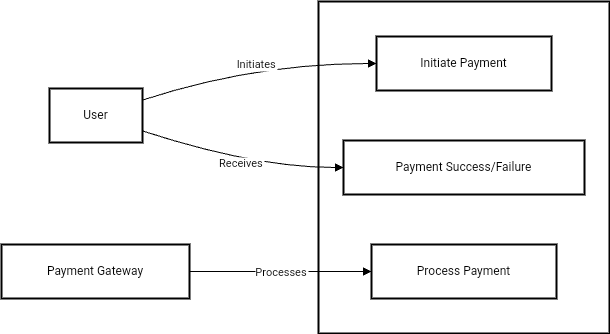
\includegraphics[width=0.8\textwidth]{./figures/Use Case Diagrams/3_usecase.png} % Replace with your actual Activity Diagram path
\captionof{figure}{Payment System Use Case Diagram}
\end{center}
\vspace{0.5cm}

\vspace{0.5cm}
\begin{center}
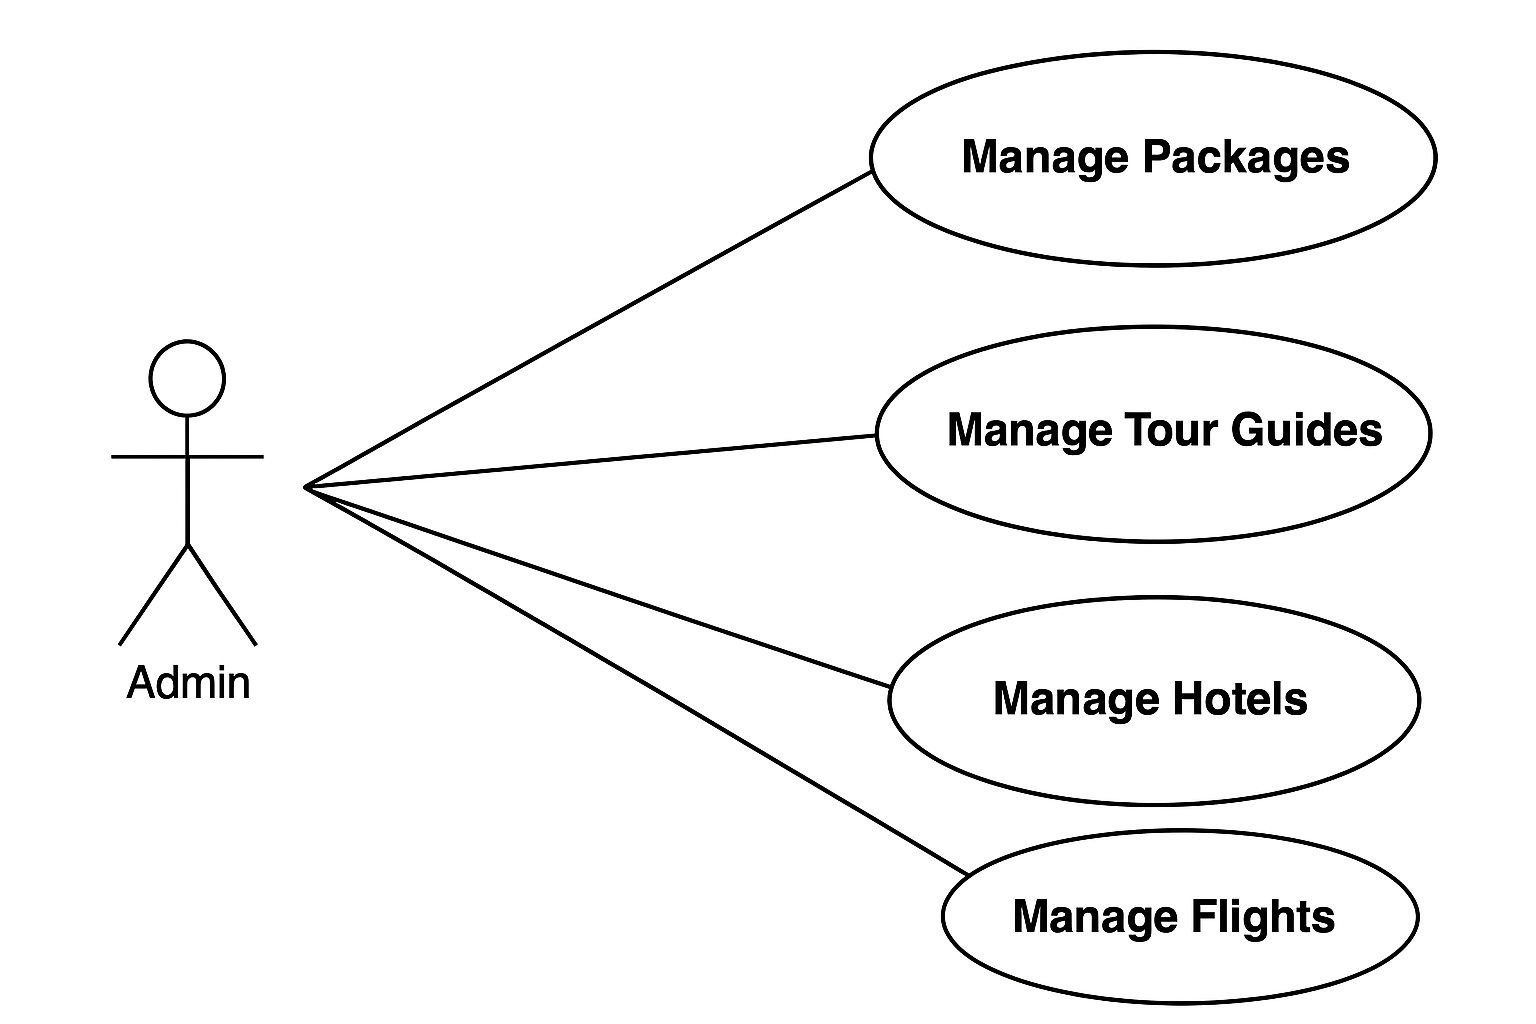
\includegraphics[width=0.8\textwidth]{./figures/Use Case Diagrams/4_crud_usecase.png} % Replace with your actual Activity Diagram path
\captionof{figure}{Admin CRUD Operation Use Case Diagram}
\end{center}
\vspace{0.5cm}


\clearpage
\chapter{Implementation Details} \label{ch: implementation}
\section{Login Component Implementation}

The login component provides secure authentication for users through both email/password and Google sign-in methods.

\subsection{State Management}
\begin{itemize}
    \item \texttt{useState} hooks for form control:
    \begin{itemize}
        \item \texttt{email}: Stores user email input
        \item \texttt{pass}: Stores password input
        \item \texttt{error}: Tracks authentication errors
    \end{itemize}
    \item Router instance for navigation control
\end{itemize}

\begin{figure}[H]
    \centering
    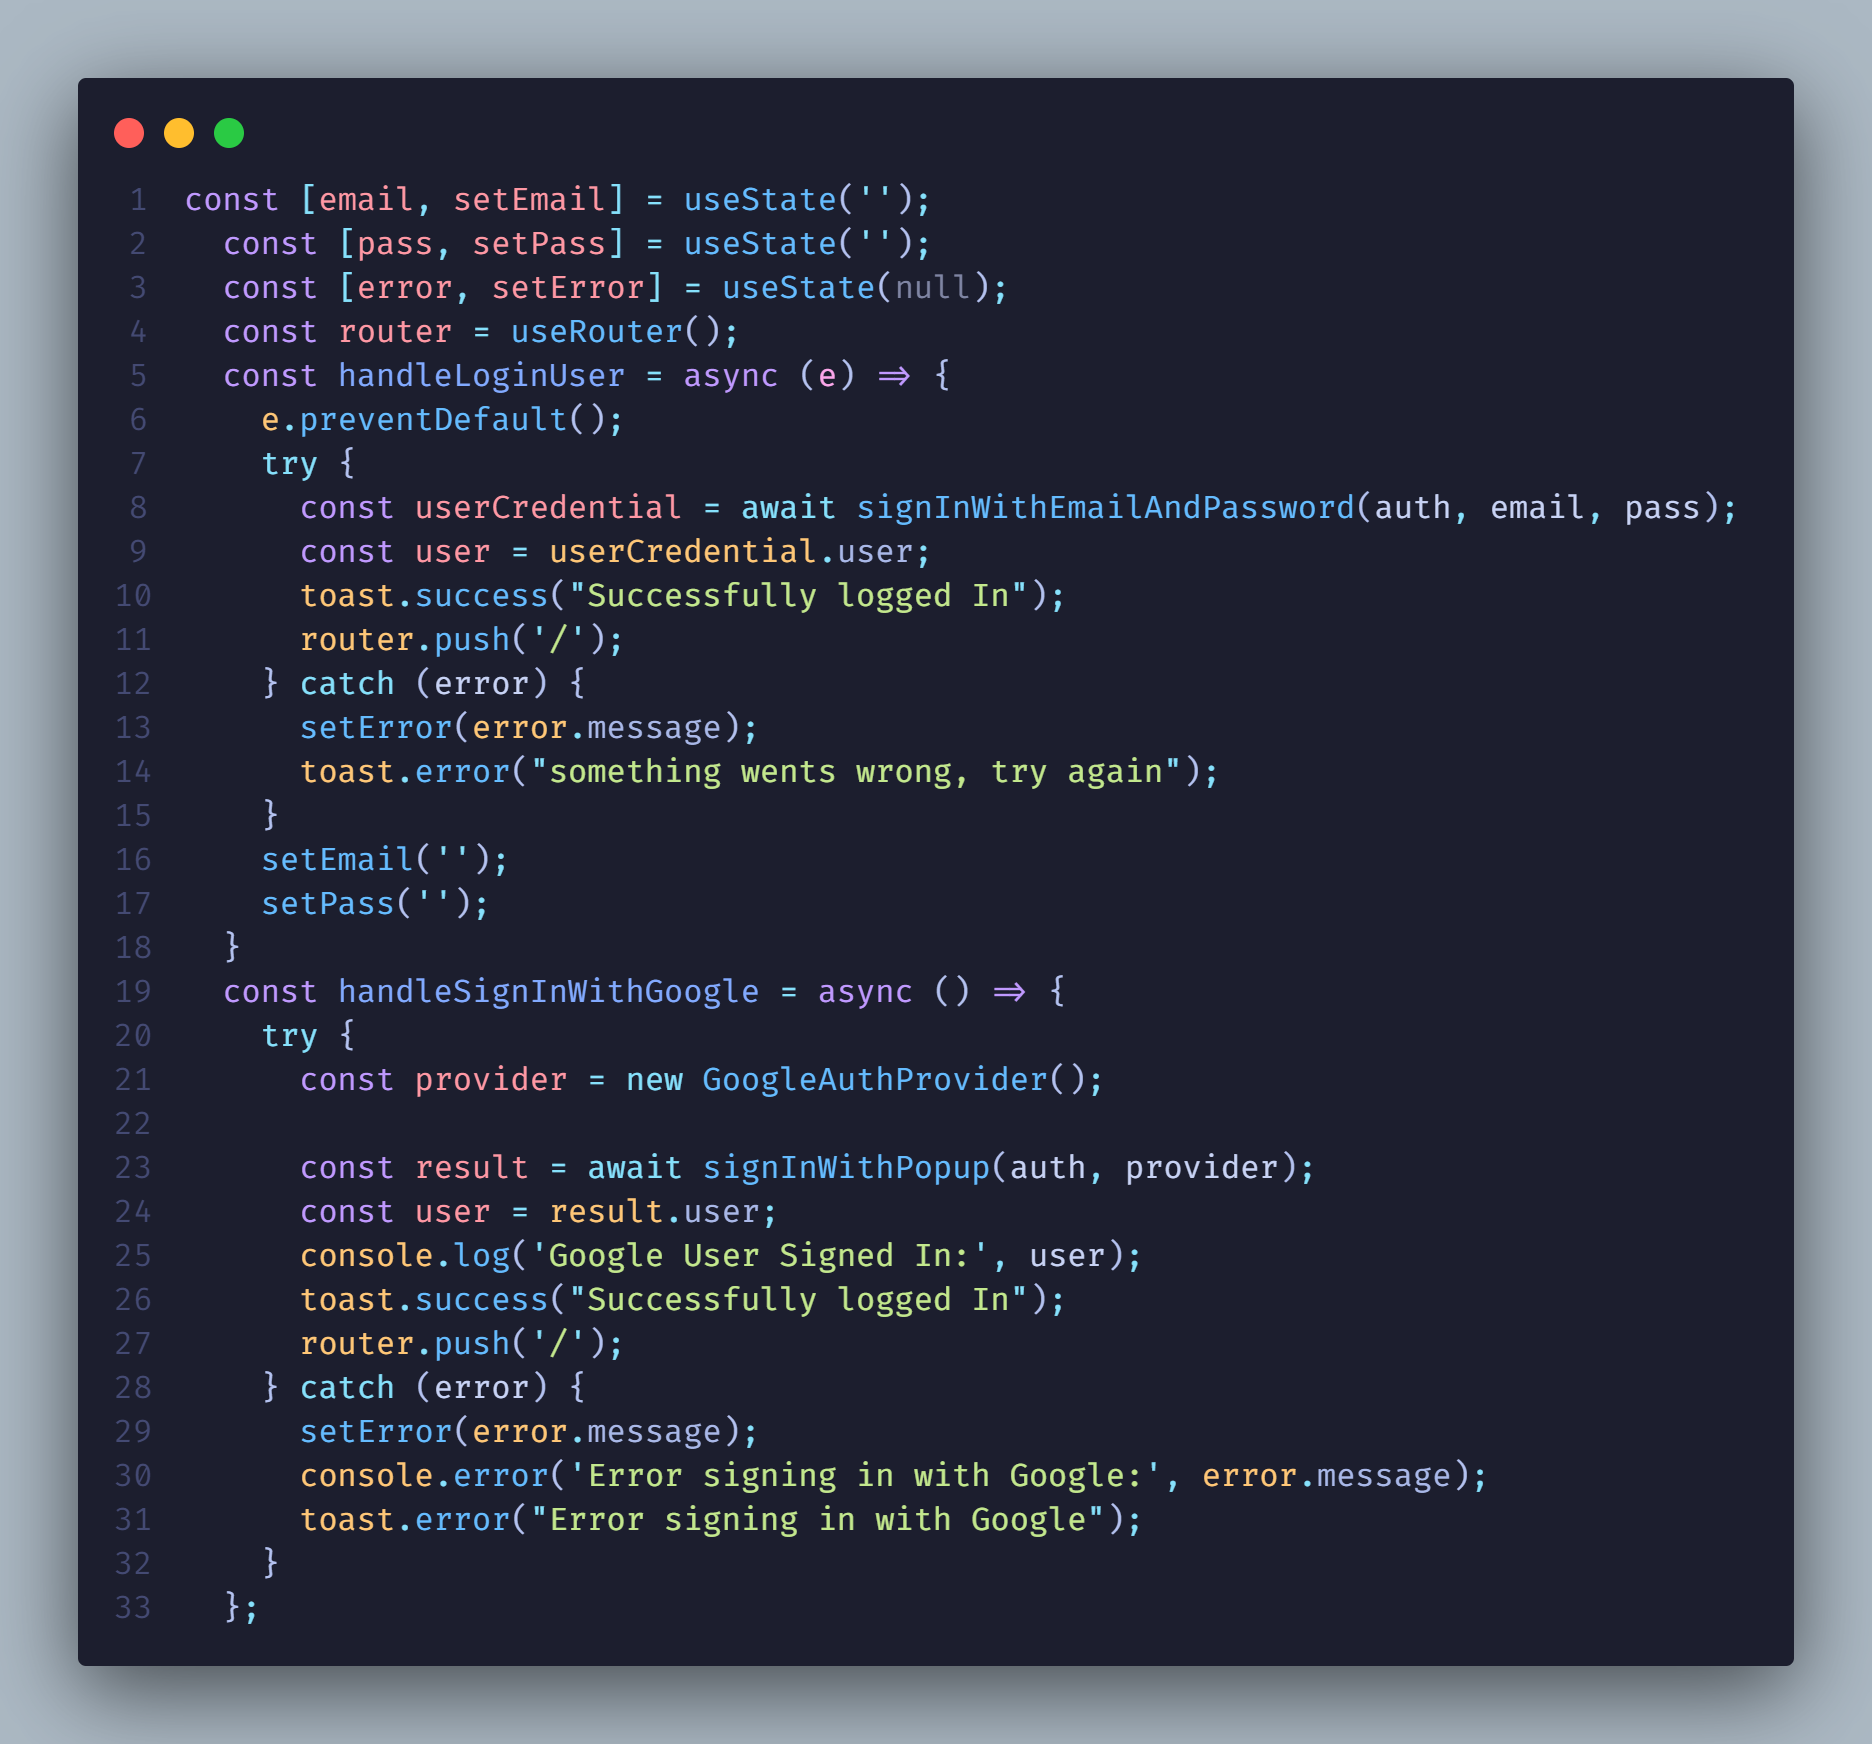
\includegraphics[width=0.9\textwidth]{./figures/implementation/login2.png}
    \caption{Login Component Code Structure}
    \label{fig:login_component}
\end{figure}

\subsection{Authentication Methods}
\begin{itemize}
    \item \textbf{Email/Password Login}:
    \begin{itemize}
        \item Uses Firebase's \texttt{signInWithEmailAndPassword}
        \item Success: Redirects to home page with success toast
        \item Error: Displays error message and toast notification
        \item Form reset after submission
    \end{itemize}
    
    \item \textbf{Google Sign-In}:
    \begin{itemize}
        \item Implements \texttt{signInWithPopup} with Google provider
        \item Success: Logs user data and redirects to home
        \item Error: Console logs error and shows toast notification
    \end{itemize}
\end{itemize}

\subsection{Error Handling}
\begin{itemize}
    \item Comprehensive try-catch blocks for both methods
    \item Error state updates for UI feedback
    \item Toast notifications for user feedback
    \item Console logging for development debugging
\end{itemize}

\subsection{Security Considerations}
\begin{itemize}
    \item Form reset after submission
    \item Protected routing after successful login
    \item No password persistence in state
    \item Secure Firebase authentication methods
\end{itemize}

\section{User Registration Implementation}

The signup component provides both email/password and Google-based registration functionality with comprehensive user profile management.

\subsection{State Management}
\begin{itemize}
    \item \texttt{useState} hooks for form control:
    \begin{itemize}
        \item \texttt{name}: Stores user's display name
        \item \texttt{email}: Stores email input
        \item \texttt{pass}: Stores password input
        \item \texttt{error}: Tracks registration errors
    \end{itemize}
    \item Router instance for navigation control
\end{itemize}

\begin{figure}[H]
    \centering
    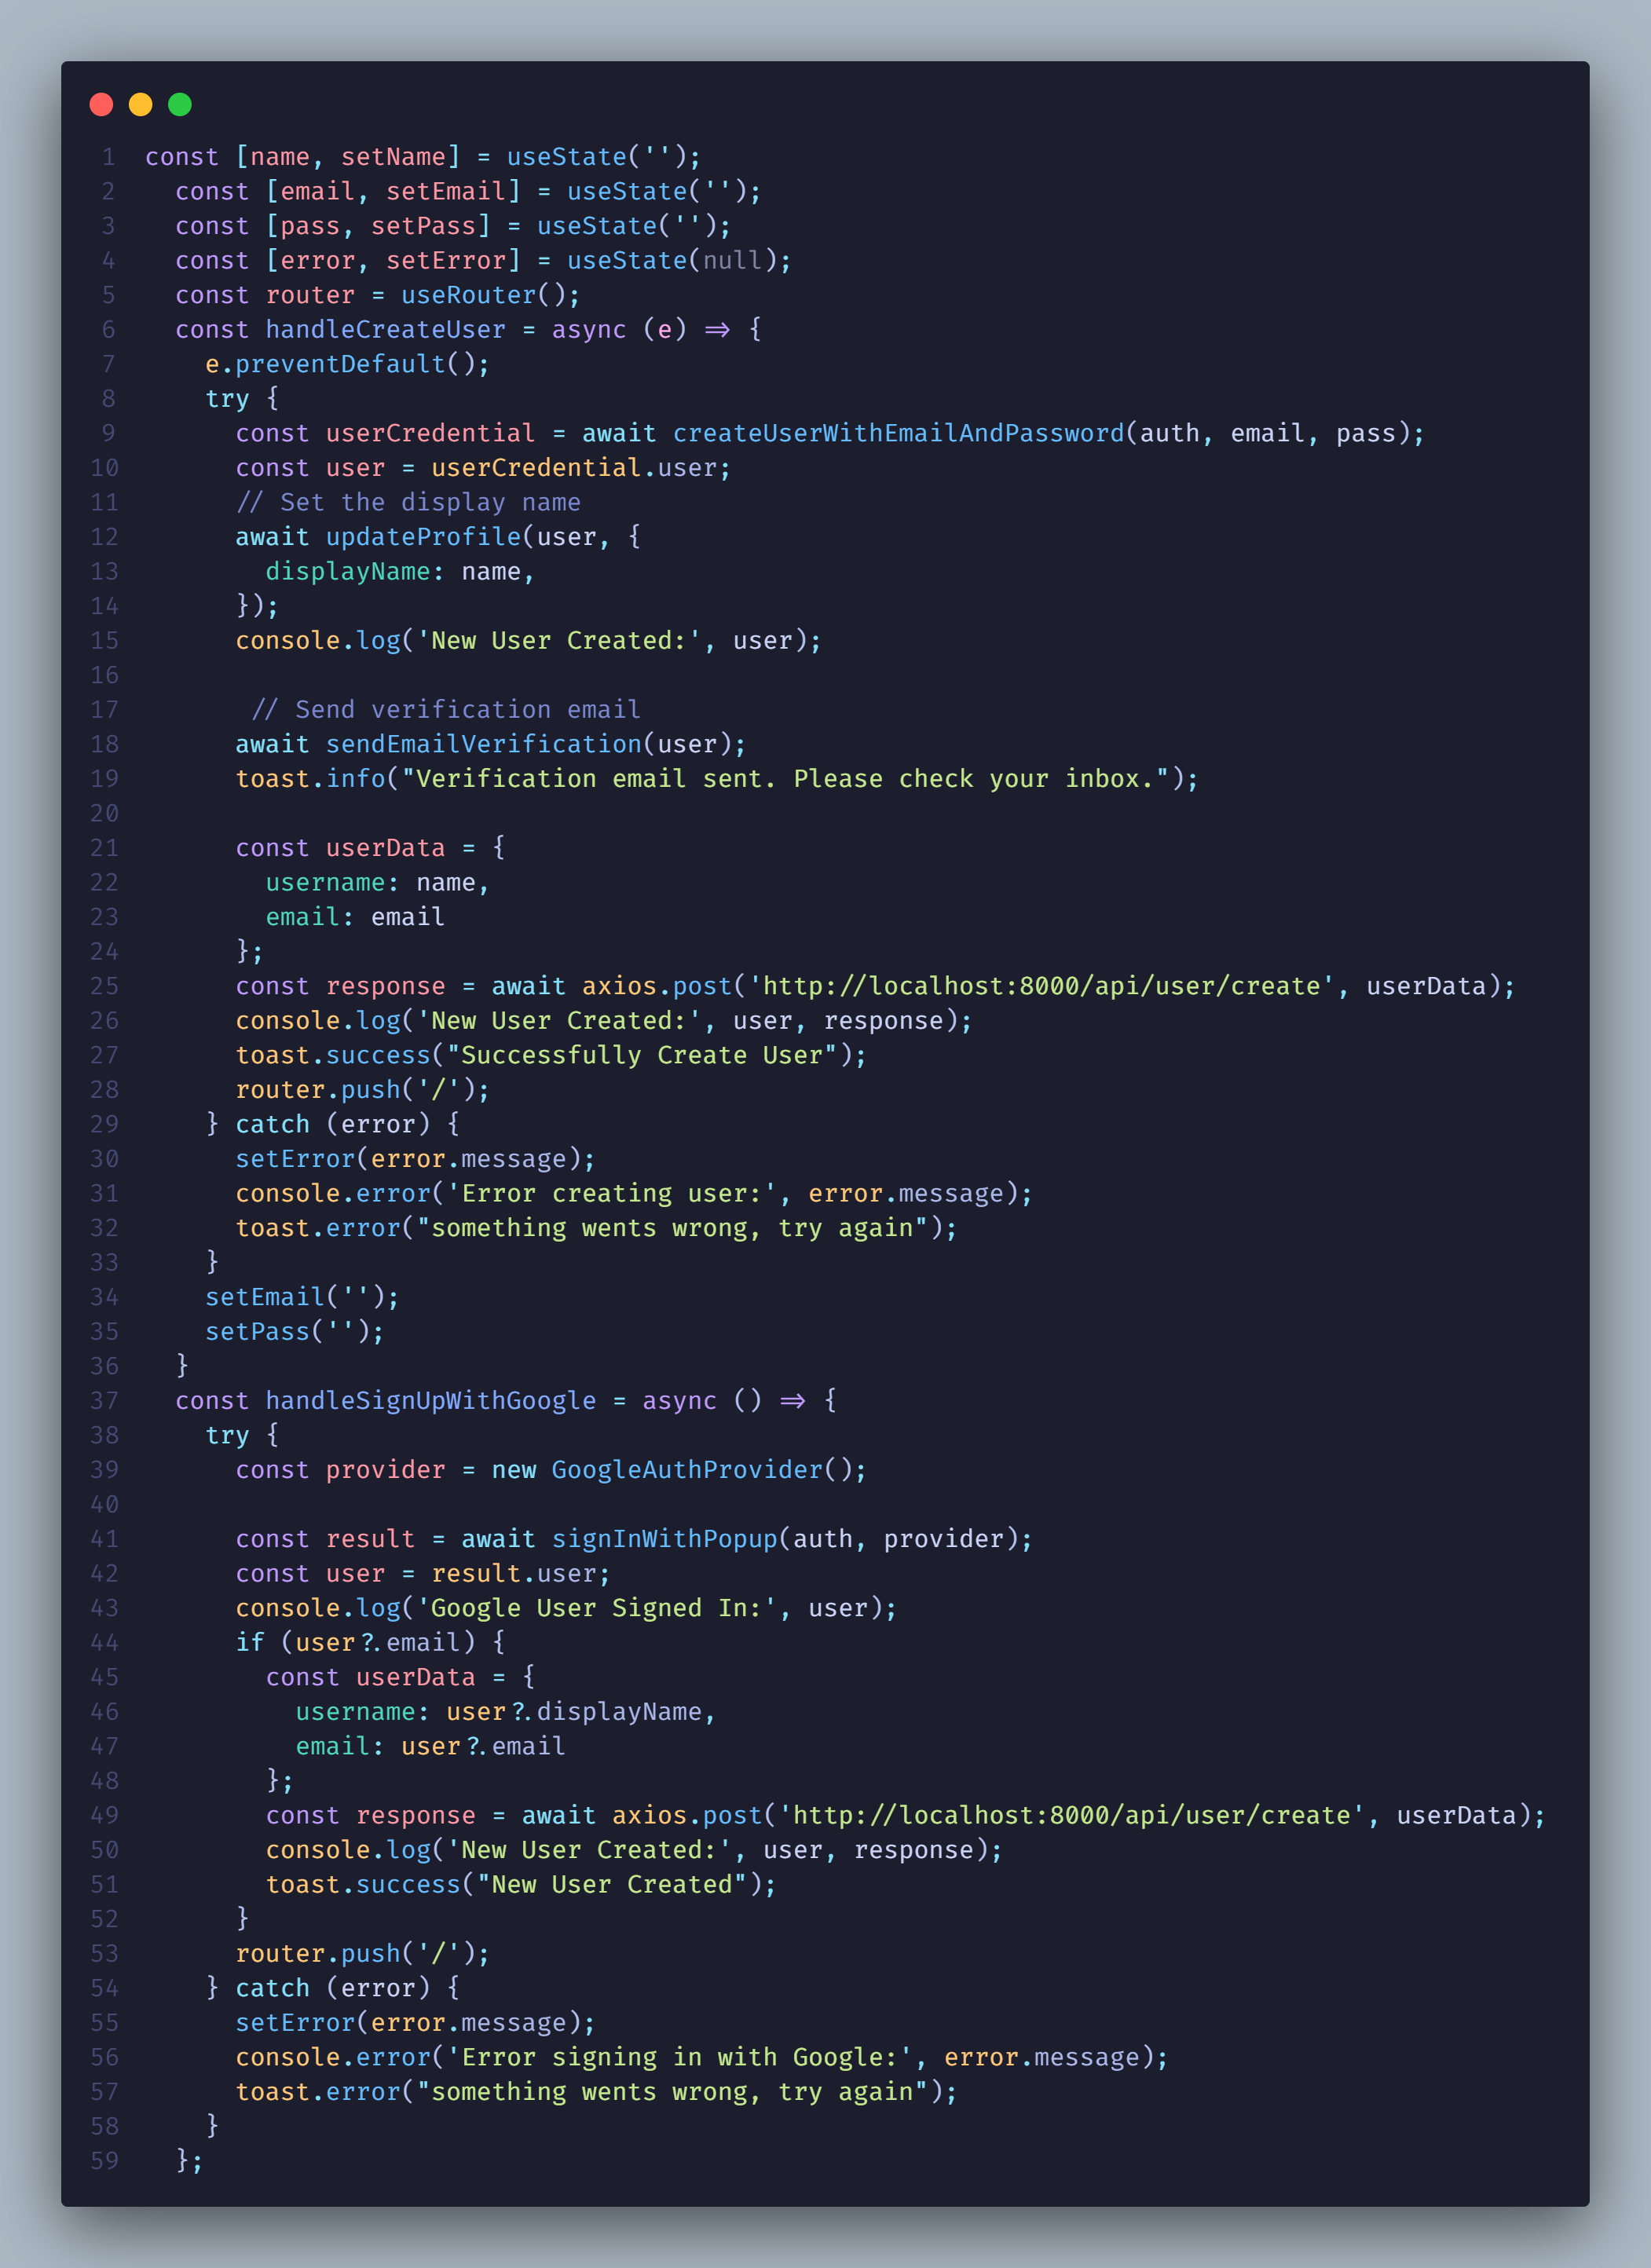
\includegraphics[width=0.9\textwidth]{./figures/implementation/signup.png}
    \caption{User Registration Code Structure}
    \label{fig:signup_component}
\end{figure}

\subsection{Registration Methods}
\begin{itemize}
    \item \textbf{Email/Password Registration}:
    \begin{itemize}
        \item Uses Firebase's \texttt{createUserWithEmailAndPassword}
        \item Sets display name via \texttt{updateProfile}
        \item Sends verification email automatically
        \item Creates backend user record via API
        \item Success: Redirects to home with success toast
    \end{itemize}
    
    \item \textbf{Google OAuth Registration}:
    \begin{itemize}
        \item Implements \texttt{signInWithPopup} with Google provider
        \item Automatically captures display name and email
        \item Creates backend user record via API
        \item Success: Redirects to home with success toast
    \end{itemize}
\end{itemize}

\subsection{Error Handling}
\begin{itemize}
    \item Comprehensive try-catch blocks for both methods
    \item Error state updates for UI feedback
    \item Toast notifications for user feedback
    \item Console logging for development debugging
    \item Form reset after email/password submission
\end{itemize}

\subsection{Security Features}
\begin{itemize}
    \item Email verification requirement
    \item Secure password handling (not persisted in state)
    \item Protected routing after successful registration
    \item Backend API integration for data consistency
\end{itemize}

\subsection{Data Flow}
\begin{itemize}
    \item Frontend to Firebase authentication
    \item Profile data to backend API (\texttt{/api/user/create})
    \item Console logging for development tracking
    \item Verification email delivery system
\end{itemize}

\section{API Routes Configuration}

The PHP code configures API routes for a travel application using Laravel, including:

\begin{itemize}
    \item User Routes: Create users, retrieve by email, assign roles
    \item Package Routes: Create, retrieve, update, delete  
    \item Hotel Routes: Create, retrieve, update, delete
    \item Flight Routes: Create, retrieve, delete
    \item Tour Guide Routes: Create, retrieve, delete
    \item Booking Routes: Create, retrieve by email
\end{itemize}

All routes use the \texttt{api} middleware group.

\begin{figure}[H]
  \centering
  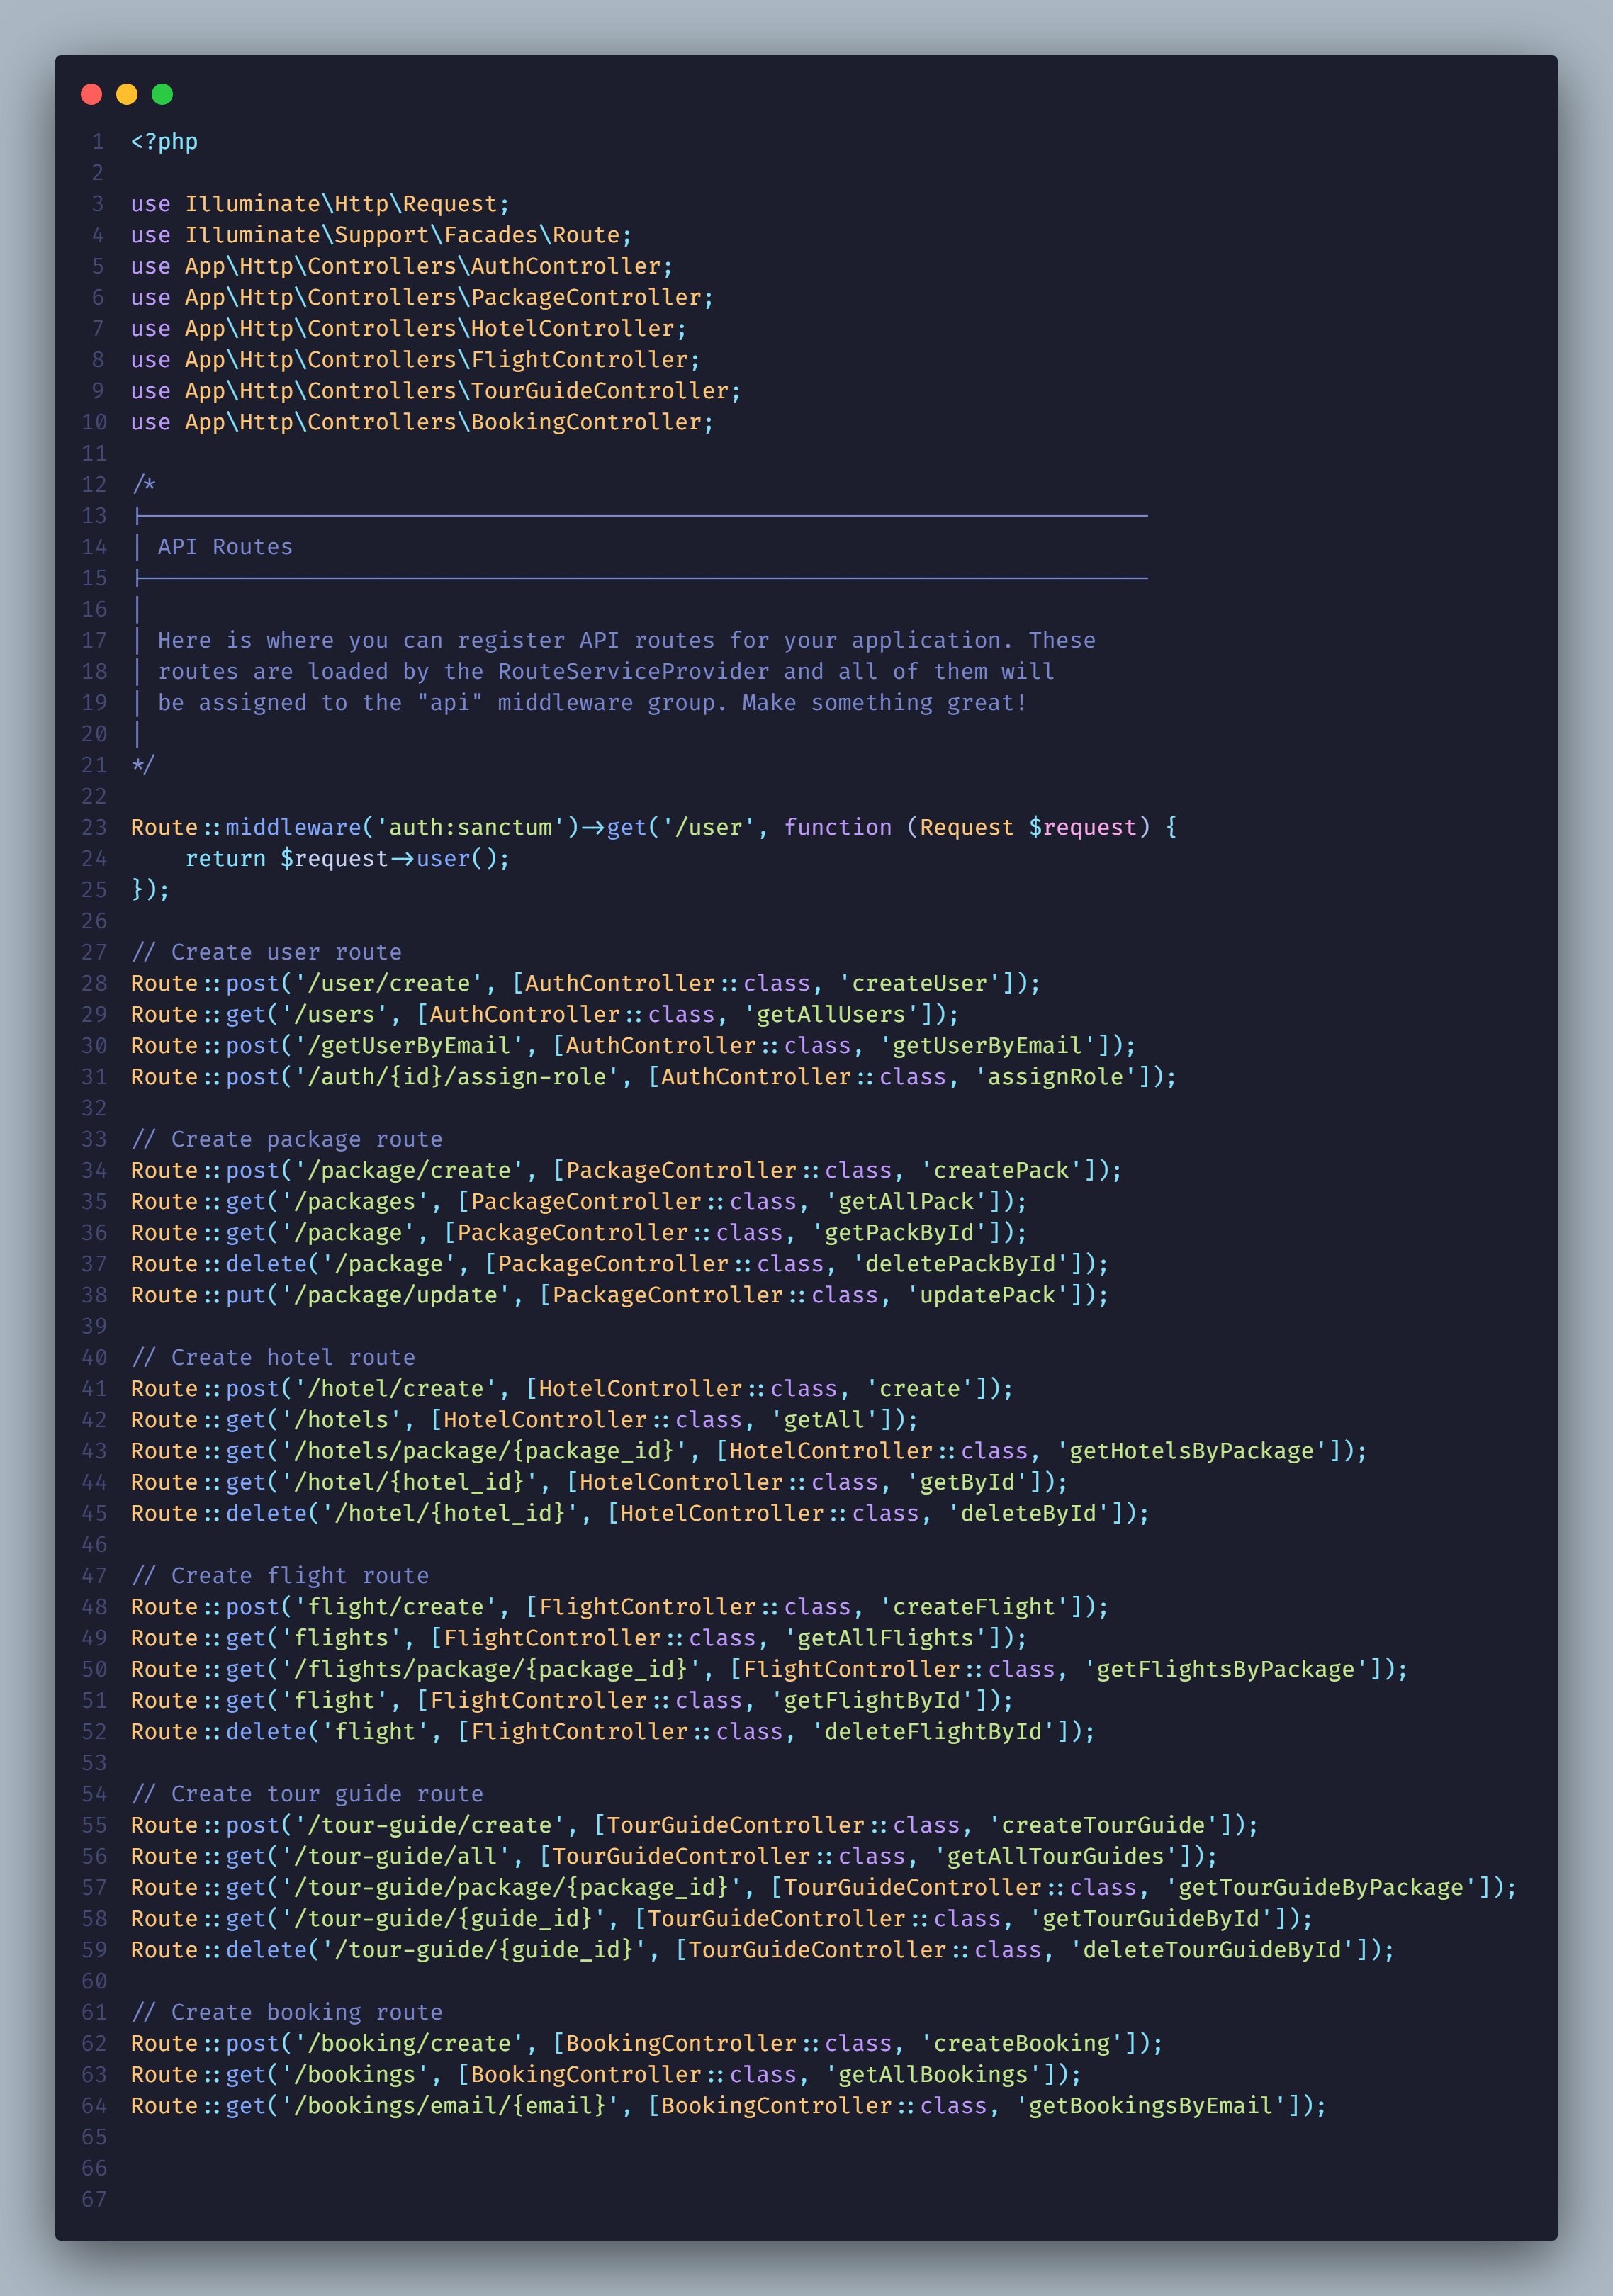
\includegraphics[width=1.0\textwidth]{./figures/implementation/api.png}
  \caption{API Routes Configuration Code Structure}
  \label{fig:api_routes}
\end{figure}

\section{Auth Controller Implementation}

The Auth Controller handles user authentication and role management operations. Key features include:

\subsection{Key Methods}
\begin{itemize}
    \item User creation with email, username, and role assignment
    \item Retrieval of all users with role information
    \item User lookup by email address
    \item Role assignment for existing users
\end{itemize}

\begin{figure}[H]
    \centering
    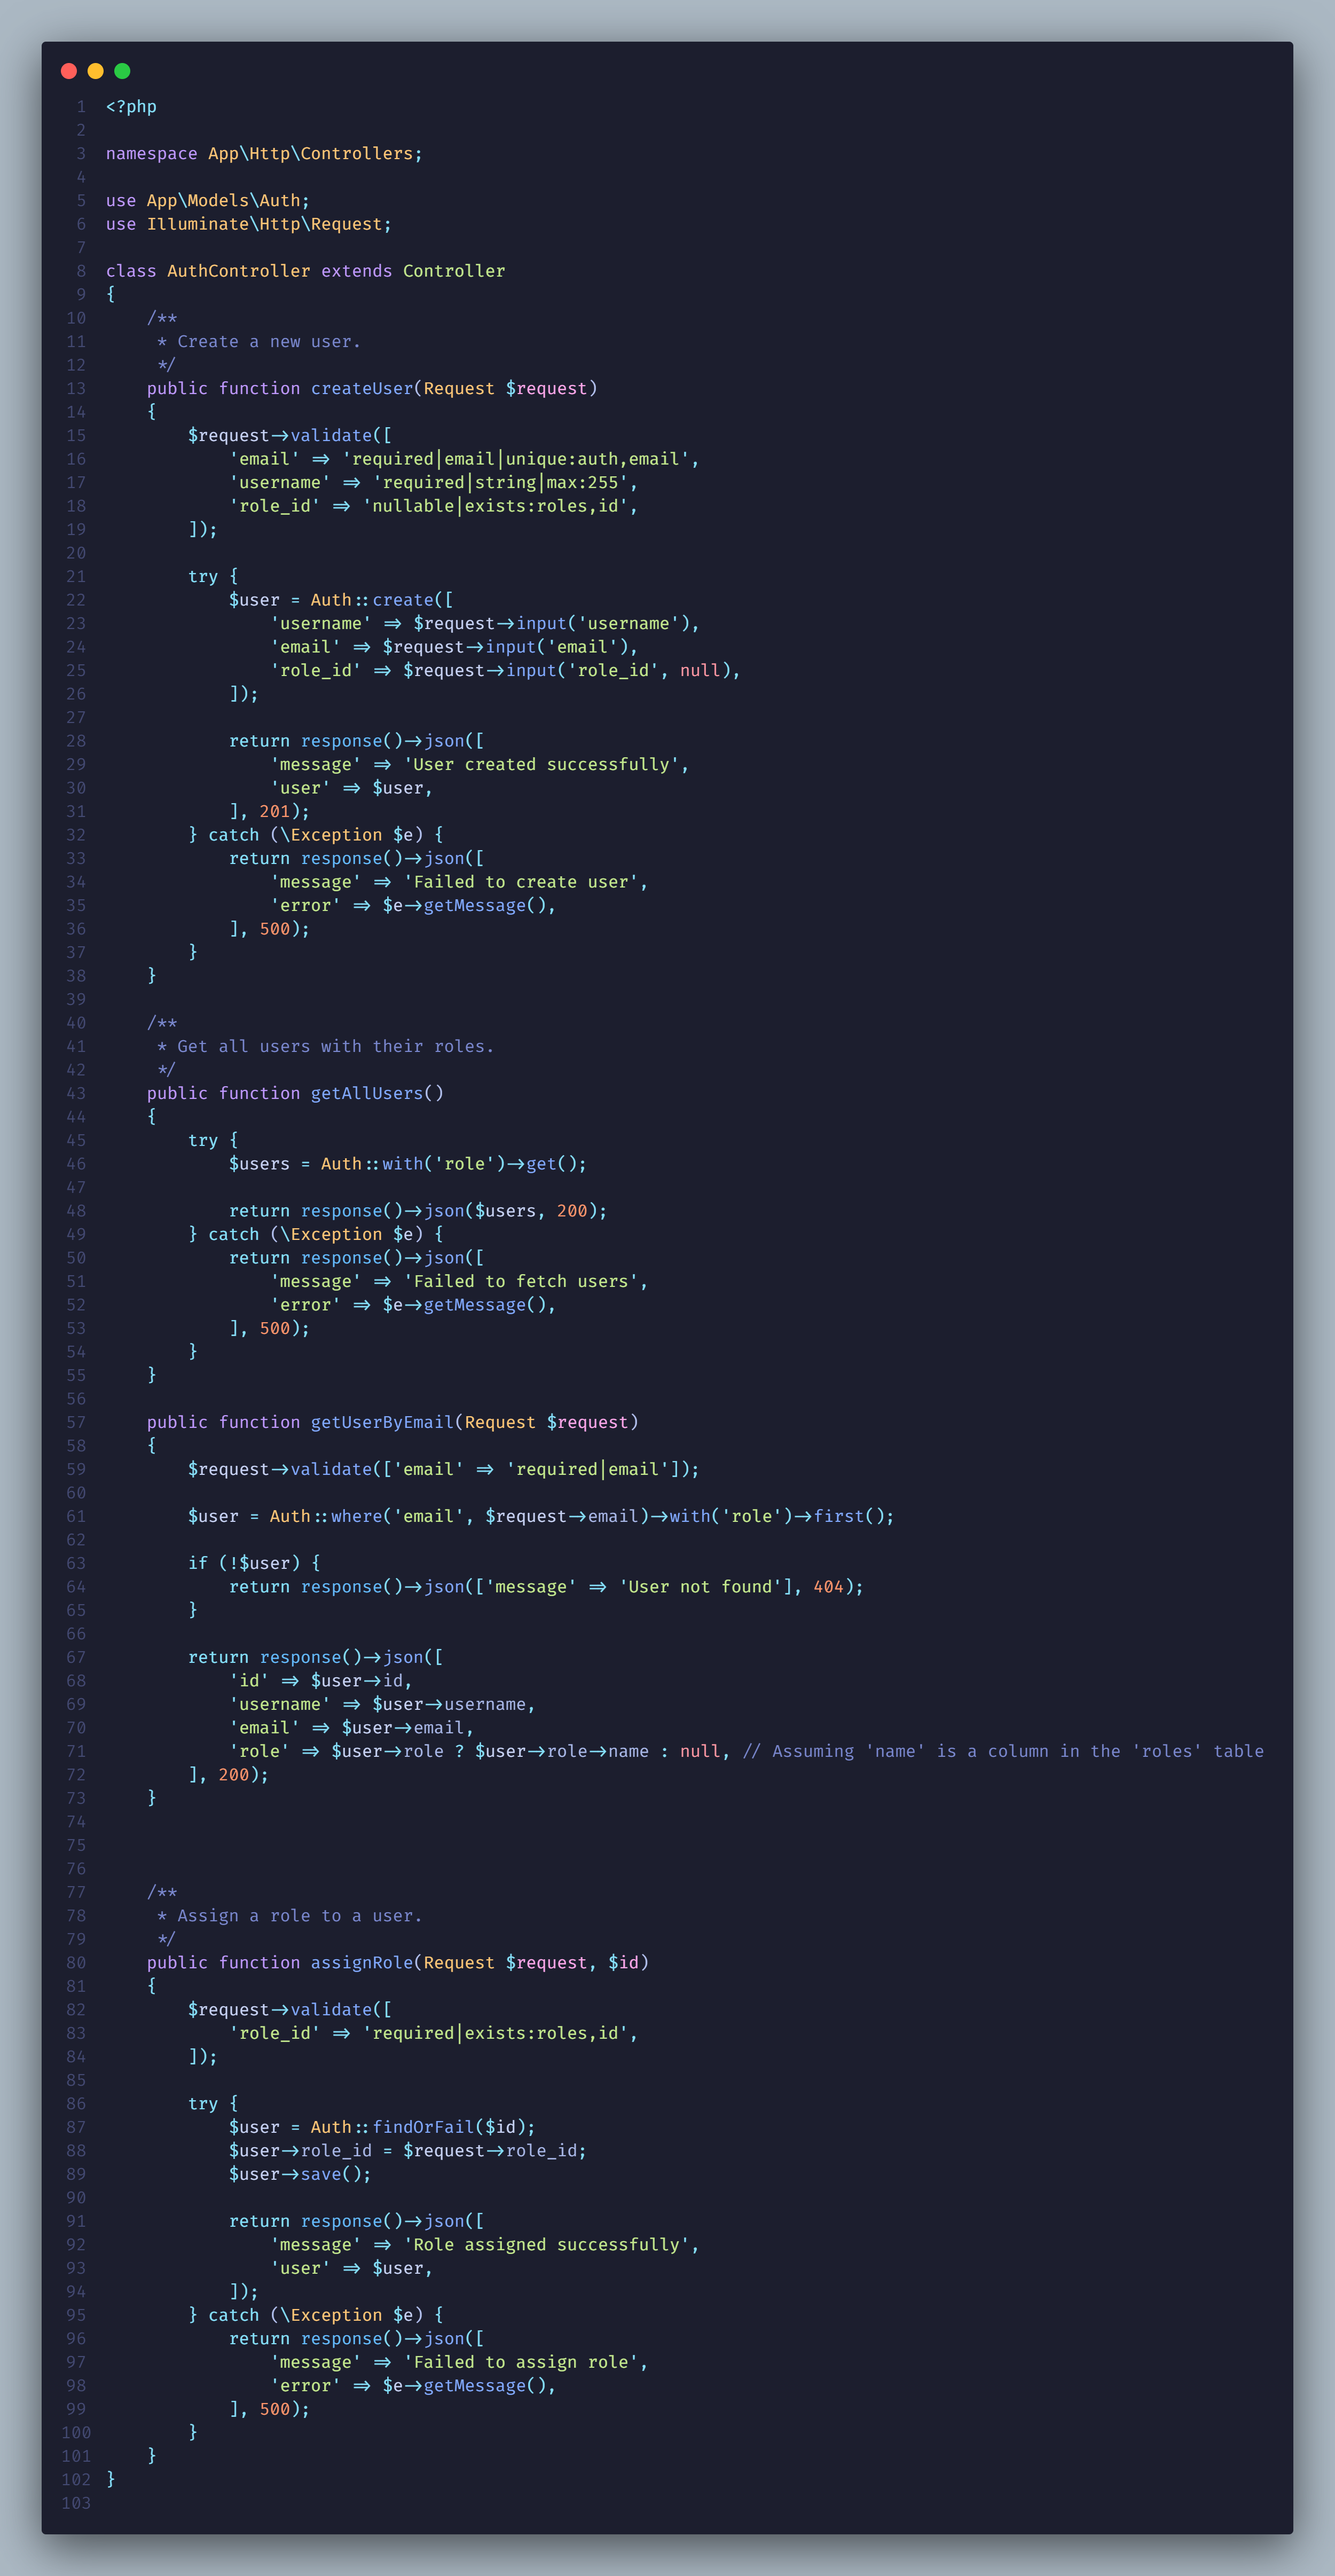
\includegraphics[width=1.0\textwidth]{./figures/implementation/Auth Controller.png}
    \caption{Auth Controller Code Structure}
    \label{fig:auth_controller}
\end{figure}

\subsection{Technical Features}
\begin{itemize}
    \item Input validation for all operations
    \item Error handling with try-catch blocks
    \item Role model integration via relationships
    \item RESTful JSON responses
\end{itemize}

\section{Package Controller Implementation}

The Package Controller manages all package-related operations in the travel application system, providing full CRUD functionality.

\subsection{Core Methods}
\begin{itemize}
    \item \texttt{createPack}: Creates new travel packages with validation
    \item \texttt{getAllPack}: Retrieves all available packages
    \item \texttt{getPackById}: Fetches specific package by ID
    \item \texttt{deletePackById}: Removes packages from the system
    \item \texttt{updatePack}: Modifies existing package details
\end{itemize}

\begin{figure}[H]
    \centering
    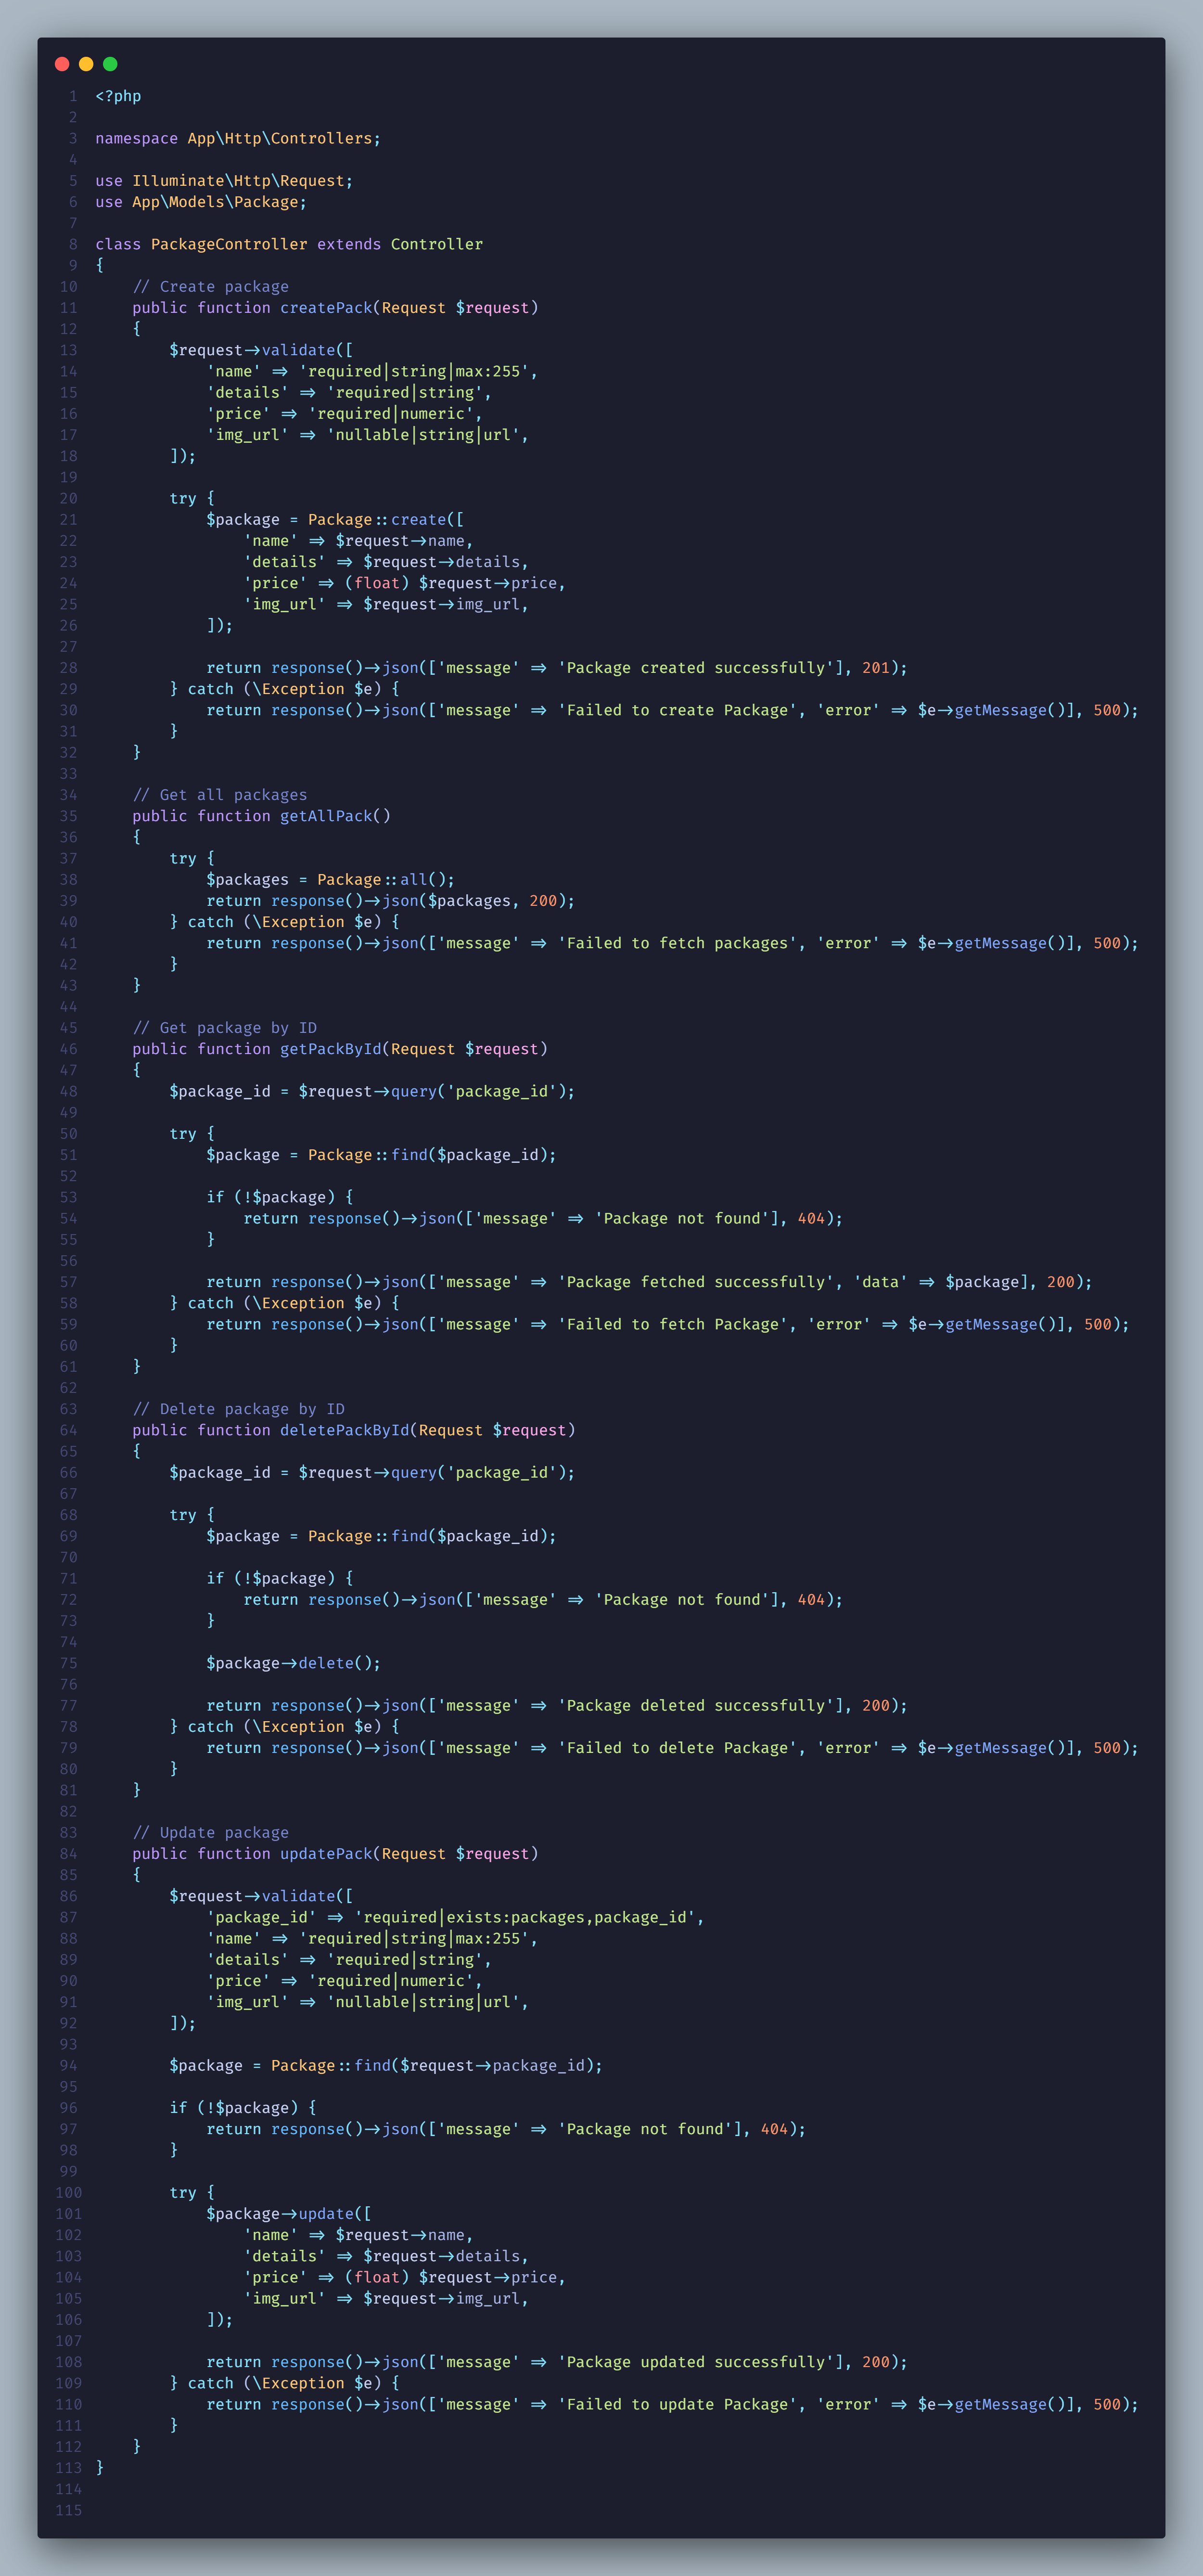
\includegraphics[width=0.9\textwidth]{./figures/implementation/Package_Controller.png}
    \caption{Package Controller Code Structure}
    \label{fig:package_controller}
\end{figure}

\subsection{Validation Rules}
\begin{itemize}
    \item Required fields:
    \begin{itemize}
        \item Package name (max 255 characters)
        \item Detailed description
        \item Price (minimum 1.0)
    \end{itemize}
    \item Optional image URL with URL validation
    \item Package ID validation for update operations
\end{itemize}

\subsection{Error Handling}
\begin{itemize}
    \item Comprehensive try-catch blocks for all operations
    \item Specific HTTP status codes:
    \begin{itemize}
        \item 200: Successful operations
        \item 400: Package not found
        \item 500: Server errors
    \end{itemize}
    \item Detailed error messages in JSON responses
\end{itemize}

\subsection{Data Processing}
\begin{itemize}
    \item Automatic price conversion to float
    \item Conditional image URL handling
    \item Proper type casting for all inputs
    \item Database transaction safety
\end{itemize}

\subsection{API Responses}
\begin{itemize}
    \item Consistent JSON response structure
    \item Success messages for all operations
    \item Error details included in failure cases
    \item Data payload for retrieval operations
\end{itemize}

\section{Booking Management System}

The booking management system handles comprehensive data processing for travel reservations. The system architecture follows a structured computer process model to ensure reliable data handling.

\subsection{Core Processes}
\begin{itemize}
    \item Data representation and information processing
    \item Comprehensive data management and tracking
    \item Flexible data modification capabilities
\end{itemize}

\begin{figure}[H]
    \centering
    
\includegraphics[width=0.9\textwidth]{./figures/implementation/booked.png}
    \caption{Booking System Code Structure}
    \label{fig:booking_system}
\end{figure}

\subsection{Key Features}
\begin{itemize}
    \item 20 modular processing components for different scenarios
    \item Uniform data handling architecture across all modules
    \item Standardized process for information representation
    \item Consistent data modification interfaces
\end{itemize}

\subsection{Technical Implementation}
The system implements:
\begin{itemize}
    \item Reusable process templates for various booking scenarios
    \item Data validation at each processing stage
    \item Audit trails for all data modifications
    \item Scalable architecture for high transaction volumes
\end{itemize}

\section{Booking Controller Implementation}

The Booking Controller manages all booking-related operations in the travel application system, providing essential CRUD functionality and query capabilities.

\subsection{Core Methods}
\begin{itemize}
    \item \texttt{createBooking}: Creates new bookings with comprehensive validation
    \item \texttt{getAllBookings}: Retrieves all booking records
    \item \texttt{getBookingsByEmail}: Finds bookings associated with a specific email
\end{itemize}

\begin{figure}[H]
    \centering
    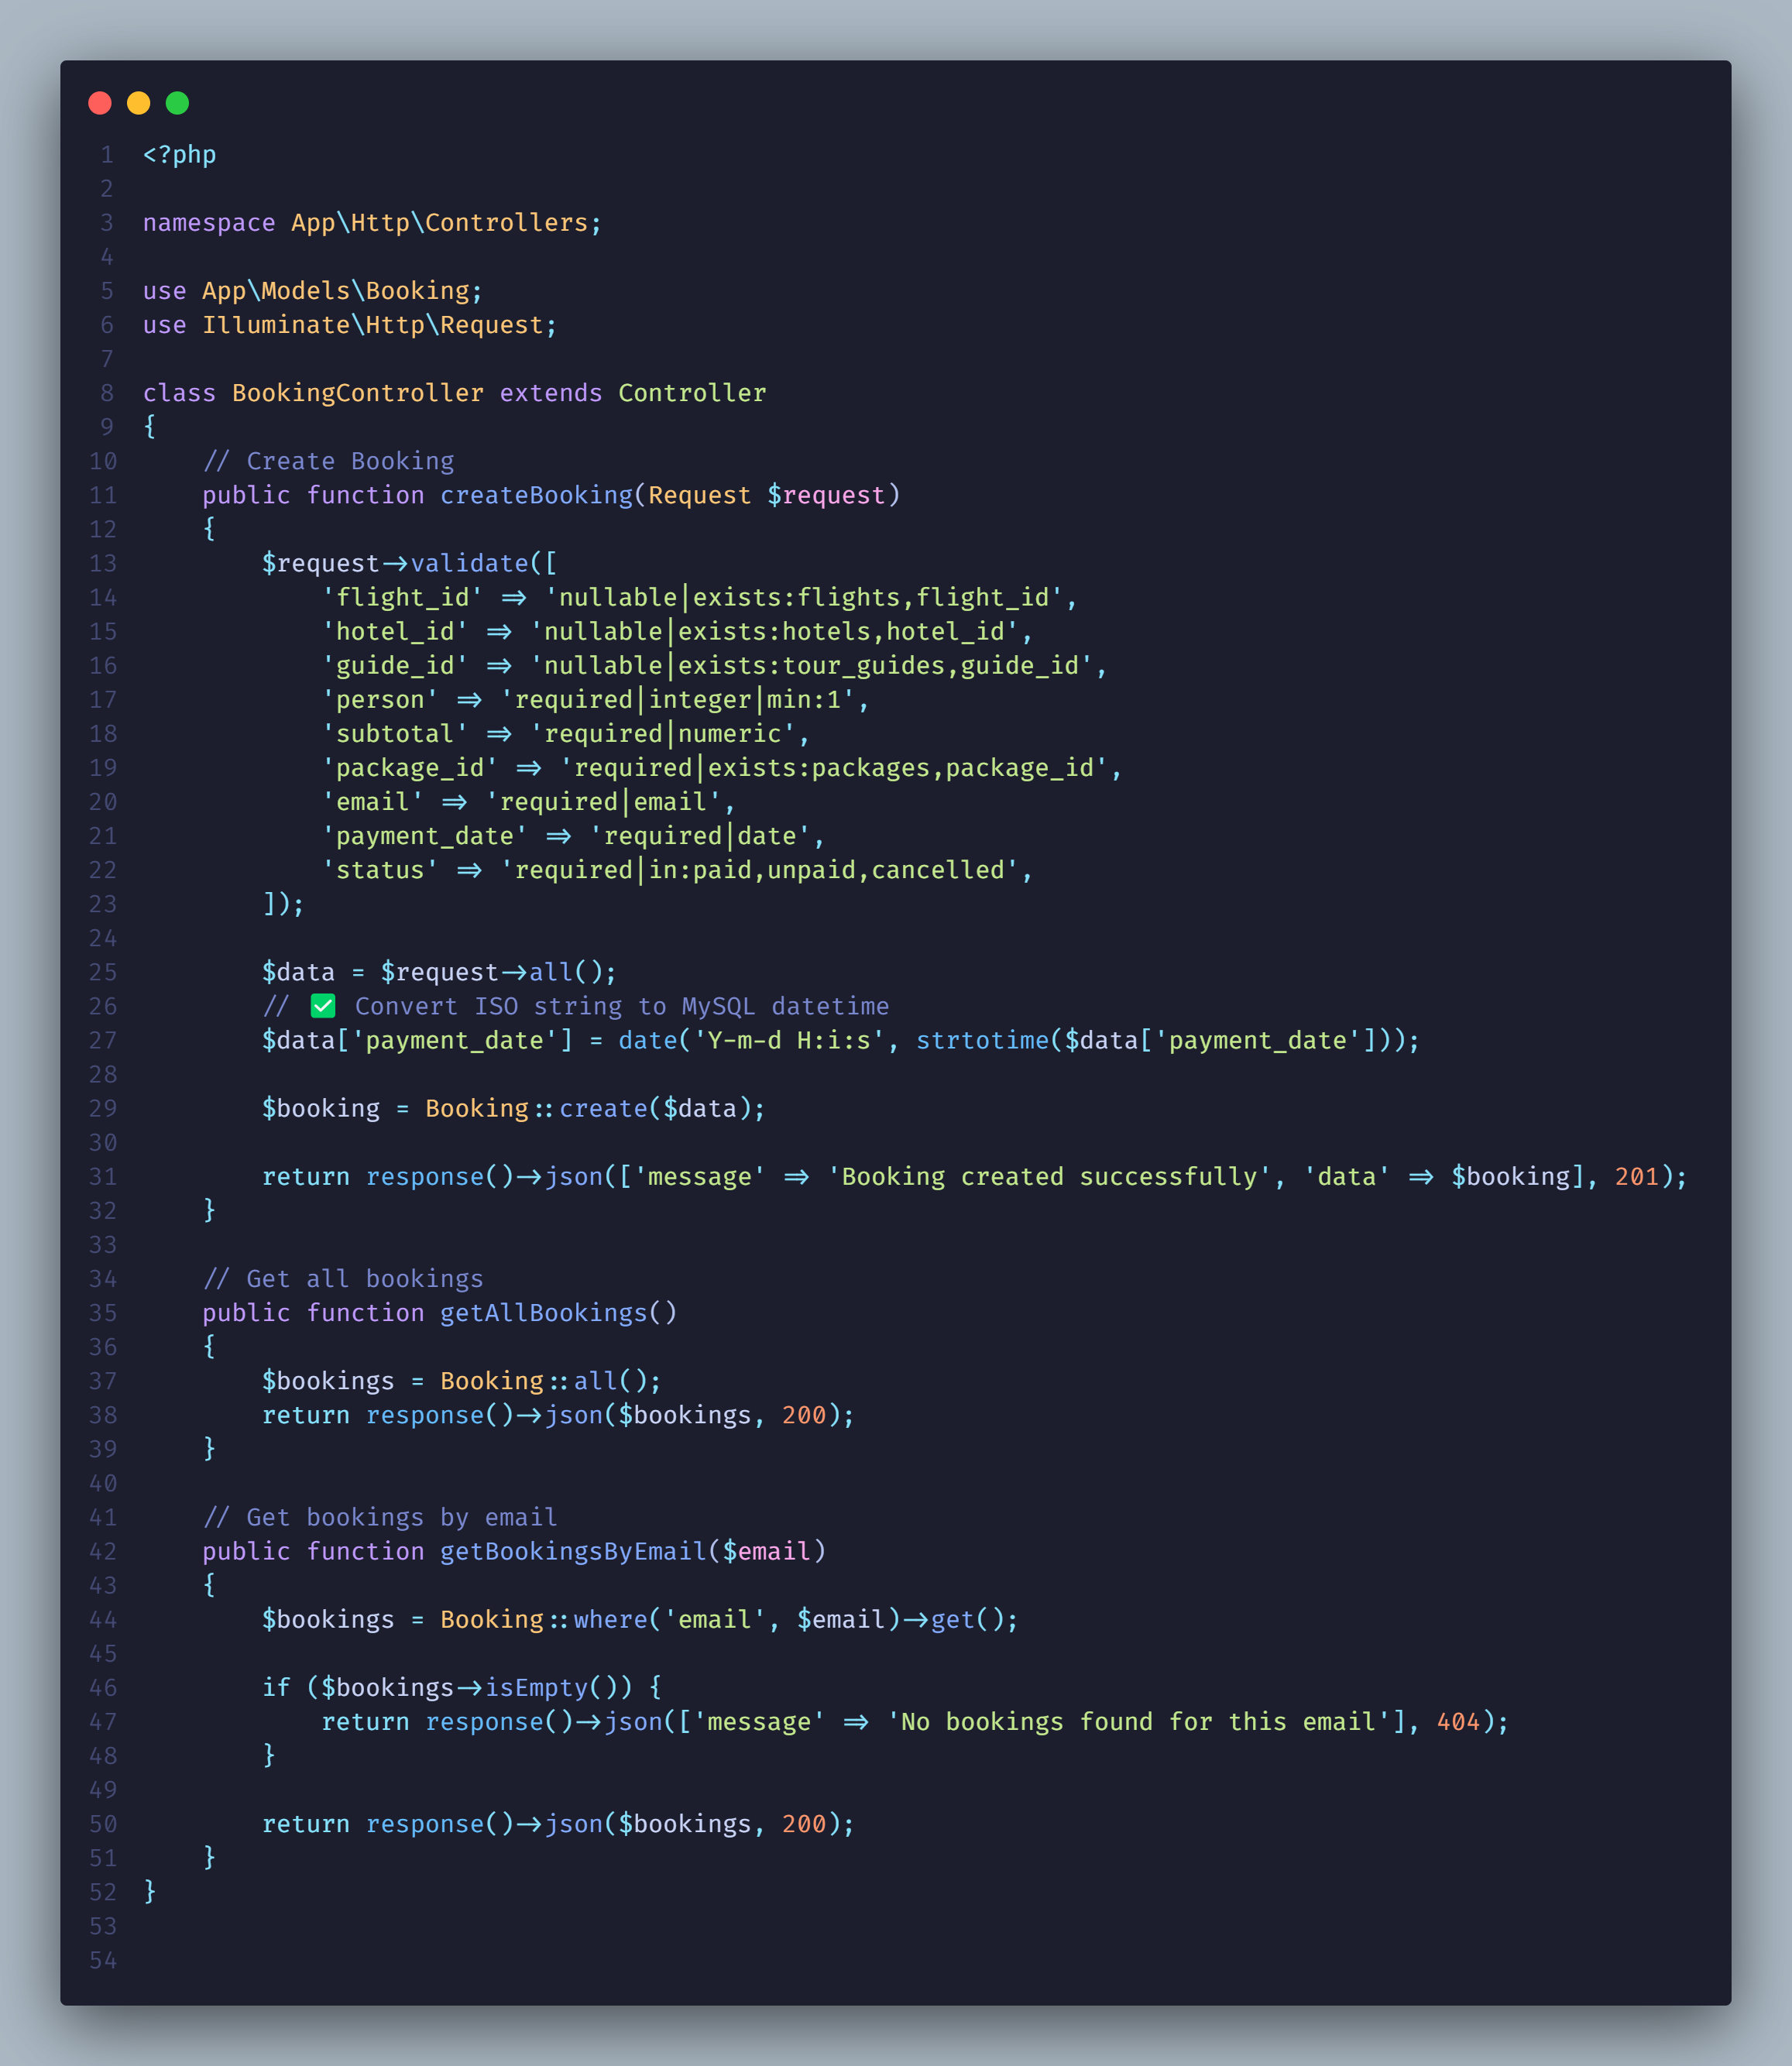
\includegraphics[width=0.9\textwidth]{./figures/implementation/Booking_Controller.png}
    \caption{Booking Controller Code Structure}
    \label{fig:booking_controller}
\end{figure}

\subsection{Technical Specifications}
\begin{itemize}
    \item \textbf{Validation Rules}:
    \begin{itemize}
        \item Foreign key checks for flights, hotels, and tour guides
        \item Required fields for person count, subtotal, and package
        \item Email format validation
        \item Payment date formatting (ISO to MySQL datetime)
        \item Status enumeration checking
    \end{itemize}
    
    \item \textbf{Data Handling}:
    \begin{itemize}
        \item Automatic date format conversion
        \item JSON response standardization
        \item Proper HTTP status codes (201, 200, 404)
    \end{itemize}
    
    \item \textbf{Error Handling}:
    \begin{itemize}
        \item Empty result detection for email queries
        \item Automatic validation error responses
    \end{itemize}
\end{itemize}

\subsection{Database Relations}
The controller interfaces with multiple database tables:
\begin{itemize}
    \item \texttt{flights} (optional relation)
    \item \texttt{hotels} (optional relation)
    \item \texttt{tour\_guides} (optional relation)
    \item \texttt{packages} (required relation)
\end{itemize}

\section{Frontend Booking Implementation}

The booking frontend interface provides users with a dynamic form to create travel reservations, integrating with multiple backend APIs.

\subsection{State Management}
\begin{itemize}
    \item \texttt{useState} hooks for all form fields:
    \begin{itemize}
        \item User email (auto-populated from authentication)
        \item Person count (default: 1)
        \item Flight, hotel, and tour guide selections
        \item Package selection from URL parameters
        \item Loading and processing states
    \end{itemize}
    \item Pagination control via \texttt{page} state
\end{itemize}

\begin{figure}[H]
    \centering
    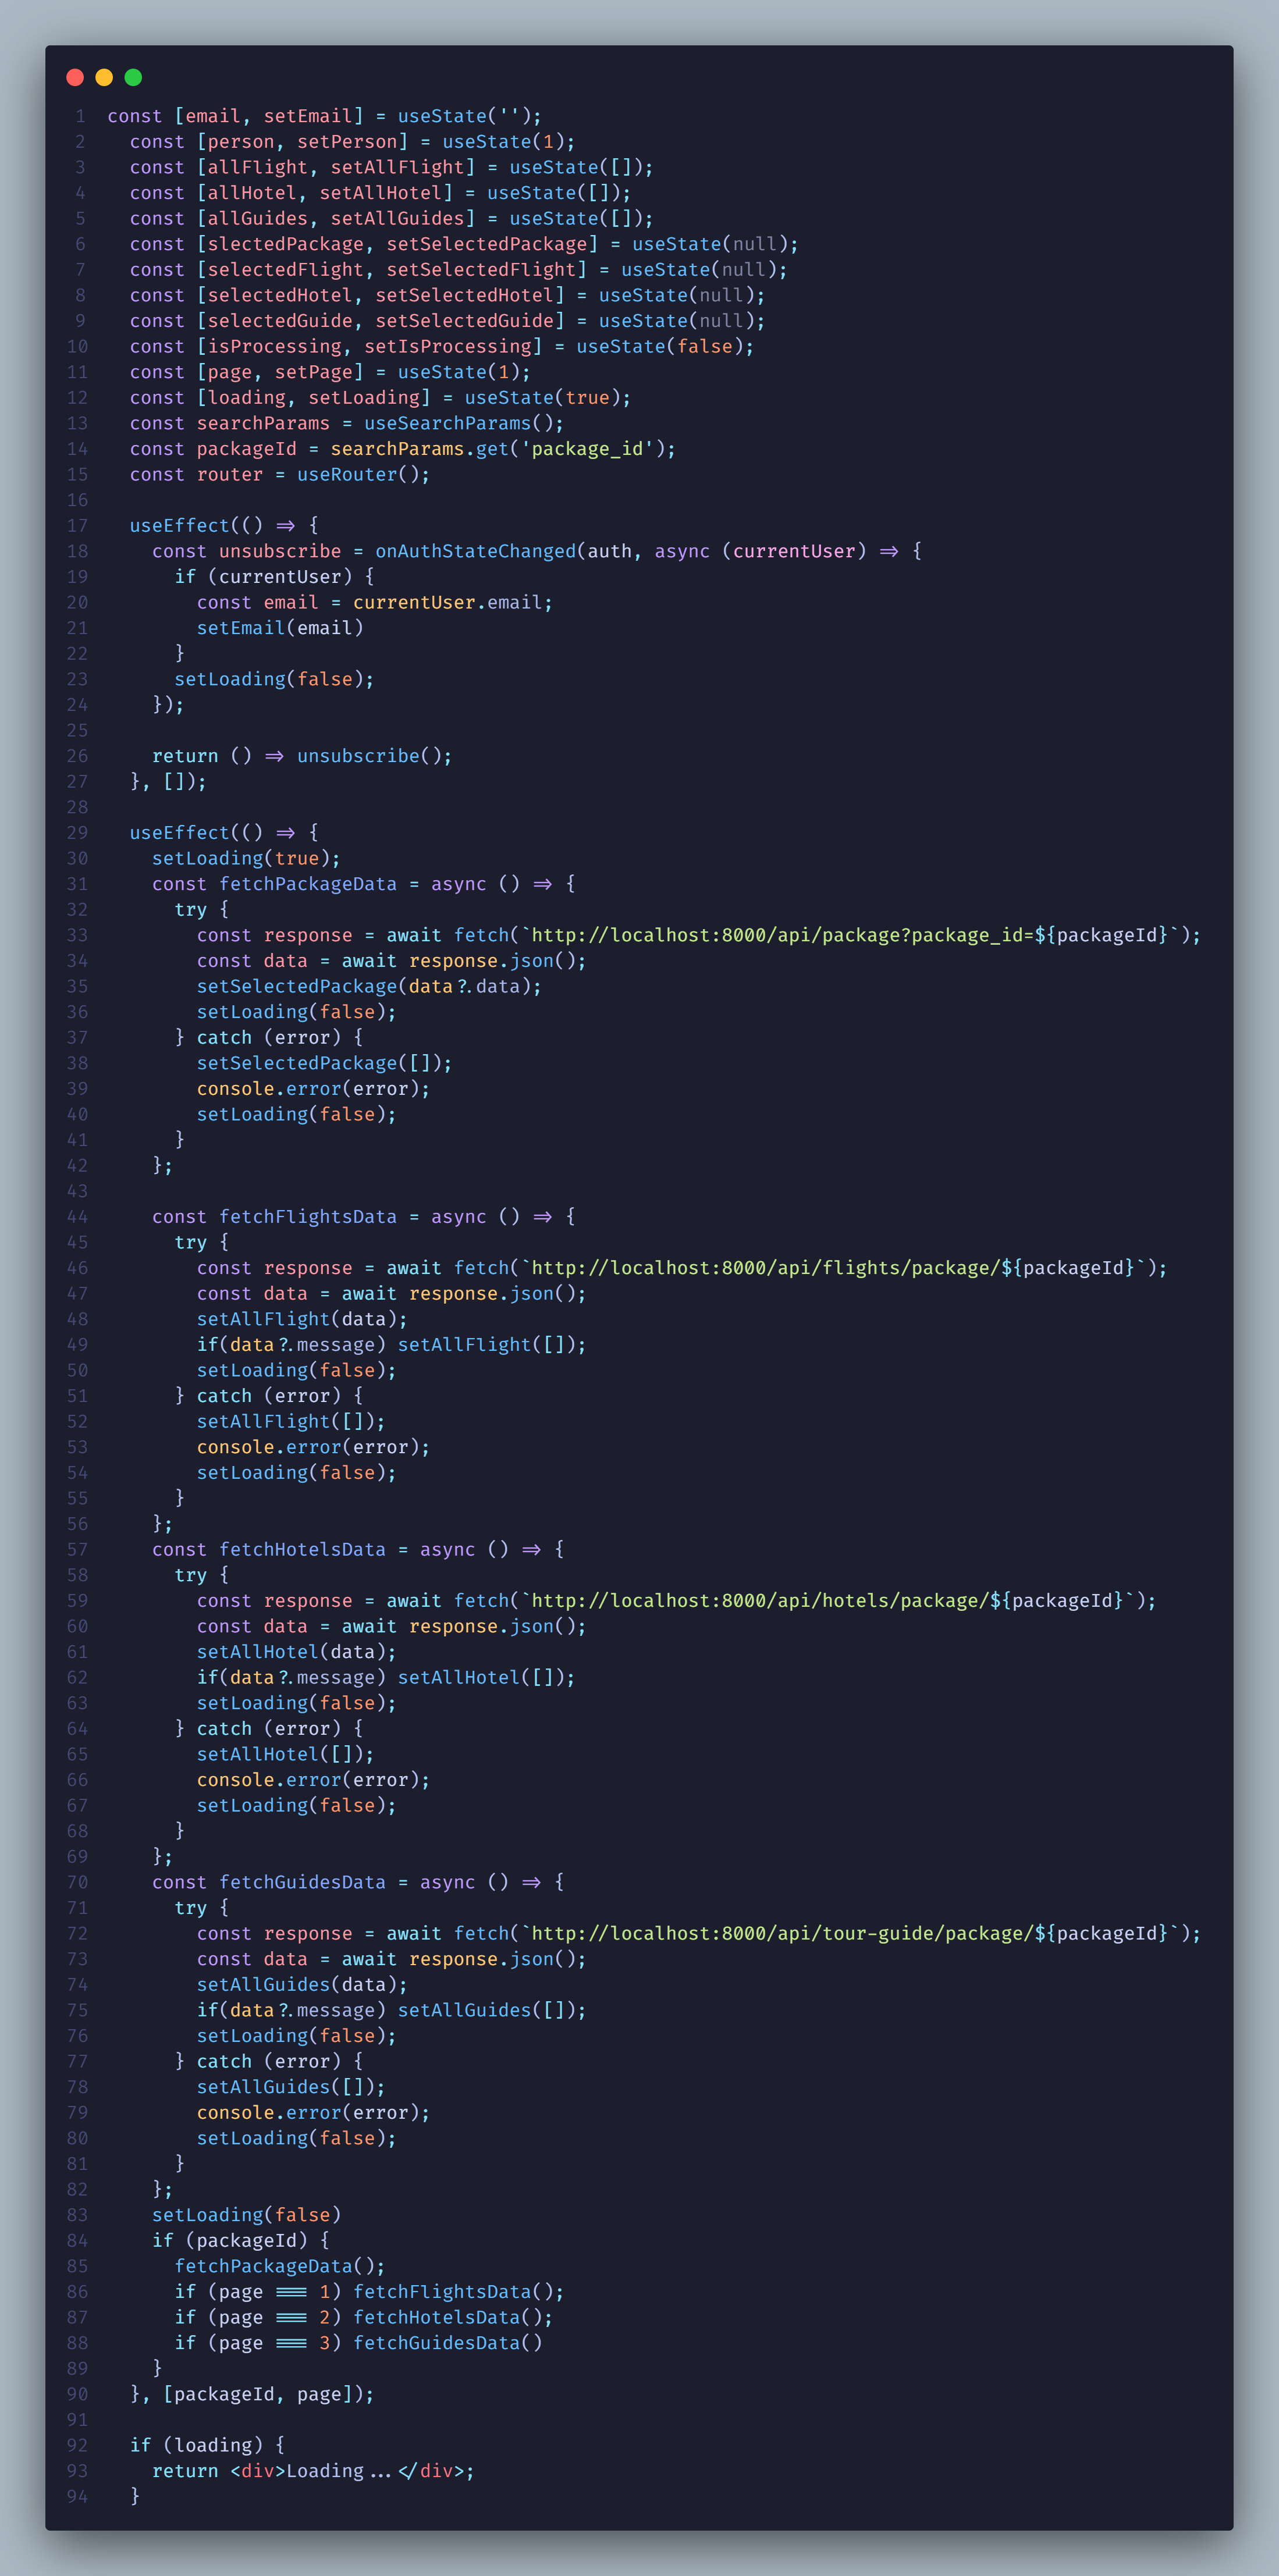
\includegraphics[width=0.9\textwidth]{./figures/implementation/booking-frontend.png}
    \caption{Booking Frontend State Management and API Integration Code Structure}
    \label{fig:booking_frontend}
\end{figure}

\subsection{API Integration}
\begin{itemize}
    \item \textbf{Data Fetching}:
    \begin{itemize}
        \item Package details from \texttt{/api/package}
        \item Available flights from \texttt{/api/flights/package}
        \item Available hotels from \texttt{/api/hotels/package}
        \item Available guides from \texttt{/api/tour-guide/package}
    \end{itemize}
    
    \item \textbf{Authentication}:
    \begin{itemize}
        \item Automatic email capture from authenticated users
        \item Loading state management during auth checks
    \end{itemize}
\end{itemize}

\subsection{Error Handling}
\begin{itemize}
    \item Empty state handling for all API responses
    \item Error logging to console
    \item Loading state management during API calls
    \item Conditional rendering based on data availability
\end{itemize}

\subsection{Component Behavior}
\begin{itemize}
    \item Dynamic data fetching based on current page
    \item Package ID extraction from URL parameters
    \item Loading indicators during data fetch operations
    \item Conditional rendering of form sections
\end{itemize}

\clearpage
\chapter{Testing} \label{ch: testing}
\newcolumntype{L}[1]{>{\raggedright\arraybackslash}p{#1}}


\section{Testing}
To ensure the reliability and correctness of the Odyssey Travel Agency Software, a structured testing methodology was followed throughout the development lifecycle. This methodology included four primary types of testing:

\begin{itemize}
    \item \textbf{Unit Testing:} Conducted on individual functions and components such as the login system, package listing, and hotel selection module. JavaScript-based unit tests were created using testing libraries like Jest.
    
    \item \textbf{Integration Testing:} Focused on verifying the interaction between modules. For example, integration of the package selection page with the booking module and the payment gateway was carefully validated.
    
    \item \textbf{System Testing:} The complete software was tested in a controlled environment to ensure it meets functional and non-functional requirements. This was done using the deployed system with sample user flows.
    
    \item \textbf{User Acceptance Testing (UAT):} Selected users were invited to test the application from a real-world user perspective. Feedback was collected and evaluated to improve usability, performance, and correctness.
\end{itemize}

\section{Unit Testing}
Unit testing was conducted to test individual modules in isolation. The main goals were to verify correctness of logic, detect early bugs, and ensure maintainability.

\begin{itemize}
    \item Each React component and backend API endpoint was tested using automated test cases.
    \item Modules like authentication, registration, tour guide assignment, and package search were tested individually.
    \item Edge cases were tested such as invalid email formats, empty form submissions, and duplicate user entries.
\end{itemize}

Sample assertion example for user registration:
\begin{verbatim}
expect(registerUser("test@mail.com", "password123")).toBeTruthy();
\end{verbatim}

\section{Integration Testing}
Integration testing was carried out to ensure seamless communication between various components.

\begin{itemize}
    \item Verified data flow from front-end forms to the backend database via the Express API.
    \item Ensured synchronization between hotel/flight selection and the final booking confirmation.
    \item Checked for error handling during API failures or slow network conditions.
\end{itemize}

For example, a package booked by the user was tested to ensure the details were stored correctly and retrievable under the user's booking history.

\section{System Testing}
System testing evaluated the behavior of the complete application. Both functional and non-functional requirements were validated.

\begin{itemize}
    \item Complete booking workflows were tested – from login to payment confirmation.
    \item Admin panel functionalities such as package CRUD operations and tour guide assignment were fully validated.
    \item Tested across multiple browsers (Chrome, Firefox, Edge) to ensure UI consistency.
\end{itemize}

All modules worked correctly when deployed via a local server using XAMPP and MySQL database integration.

\section{User Acceptance Testing}
UAT was performed with a group of 5 users including students and travelers. Their task was to use the system and provide usability feedback.

\begin{itemize}
    \item Majority found the interface intuitive and easy to navigate.
    \item Suggestions were made to improve hotel filtering and add date-based filtering in future versions.
    \item No major bugs were reported during this phase, indicating system readiness.
\end{itemize}

User feedback was recorded and considered for future iteration plans.

\section{Test Cases and Results}
A set of planned test cases were executed to validate the system’s critical functions. A sample of these test cases is summarized below:


\begin{longtable}{|L{6cm}|L{10cm}|}
    \caption{Project Information Table} \label{tab:project_info} \\
    \hline
    \textbf{Project Name} & Odyssey Travel Agency Software
    \\ \hline
    \textbf{Module Name} & Software Testing \\ \hline
    \textbf{Created By} & Hafizur Rahman Sakib and Arnab Shikder \\ \hline
    \textbf{Date of Creation} & 17.02.2024 \\ \hline
    \textbf{Date of Review} & 02.05.2025 \\ \hline
  \end{longtable}

\begin{longtable}[
    ]{
      |L{1.3cm}|L{2.2cm}|L{2.0cm}|L{2.5cm}|L{2.0cm}|L{2.2cm}|L{1.3cm}|
    }
    \caption{Comprehensive Test Case Execution Table for Odyssey Travel Agency Software} \label{tab:test_cases} \\
    \hline
    \textbf{Test Case ID} & 
    \textbf{Test Scenario} & 
    \textbf{Pre-Condition} & 
    \textbf{Test Steps} & 
    \textbf{Test Data} & 
    \textbf{Expected Result} & 
    \textbf{Status} \\
    \hline
    \endfirsthead
    \caption[]{Comprehensive Test Case Execution Table (Continued)} \\
    \hline
    \textbf{Test Case ID} & 
    \textbf{Test Scenario} & 
    \textbf{Pre-Condition} & 
    \textbf{Test Steps} & 
    \textbf{Test Data} & 
    \textbf{Expected Result} & 
    \textbf{Status} \\
    \hline
    \endhead
    \hline
    \endfoot
    \footnotesize % Use smaller font size for better fit
    TC001 & User Login & User is registered & Enter email and password, click login & Email: user@mail.com, Password: 1234 & Dashboard is shown & Pass \\ \hline
    TC002 & Add New Package & Admin is logged in & Go to ``Add Package'', fill form, click submit & Package Name: Beach Trip & Package added successfully & Pass \\ \hline
    TC003 & Invalid Booking & User logged in & Try booking a package skipping hotel selection & N/A & Error message displayed & Pass \\ \hline
    TC004 & Payment Processing & User is on payment page & Enter valid card details and submit & Card No: 4111 1111 1111 1111 & Payment confirmation message & Pass \\ \hline
    TC005 & Session Timeout & User is logged in & Wait 30 minutes without interaction & Timer: 30 mins & Session timeout message shown & Pass \\ \hline
    TC006 & Search Function & User is on homepage & Type keyword in search bar and click search & Keyword: Cox's Bazar & Related packages shown & Pass \\ \hline
    TC007 & Unauthorized Access & User is logged out & Try accessing \texttt{/admin} directly in browser & URL: /admin & Access denied or redirected to login & Pass \\ \hline
    TC008 & User Registration & N/A & Fill in name, email, password, and submit & Name: John Doe, Email: john@mail.com, Password: 1234 & Registration successful message & Pass \\ \hline
    TC009 & Password Reset & User is on login page & Click ``Forgot Password'', enter email, click submit & Email: john@mail.com & Password reset link sent to email & Pass \\ \hline
    TC010 & Edit Package & Admin is logged in & Go to ``Edit Package'', change details, click save & Package ID: 101, New Price: 5000 & Package details updated successfully & Pass \\ \hline
    TC011 & Verify User Logout & User is logged in & Click logout button & N/A & User is logged out & Pass \\ \hline
    TC012 & Invalid Payment & User is on payment page & Enter invalid card details and submit & Card No: 1234 5678 9012 3456 & Error message displayed & Pass \\ \hline
    TC013 & Change User Role & Admin is logged in & Go to user list, select user, change role, click save & User ID: 102, New Role: Admin & User role updated successfully & Pass \\ \hline
    TC014 & User Profile Update & User is logged in & Go to profile page, update name, click save & Name: John Doe $\to$ Jane Doe & Profile updated successfully & Pass \\ \hline
    TC015 & Package Filter & User is on homepage & Apply filters by location and price & Location: Cox's Bazar, Price Range: 3000--5000 & Filtered packages are shown & Pass \\ \hline
    TC016 & Cancel Booking & User is logged in, has a confirmed booking & Go to bookings, select booking, click cancel & N/A & Booking canceled successfully & Pass \\ \hline
    TC017 & Admin Login Attempt & Admin is registered & Enter invalid email or password & Email: admin@mail.com, Password: wrongpassword & Error message displayed & Pass \\ \hline
    TC018 & Package Booking Limit & User is logged in & Try booking a package with exceeded limit & Package Name: Deluxe Tour, Max Bookings: 10 & Error message displayed & Pass \\ \hline
  \end{longtable}
\section{Bug Tracking and Resolution}
Throughout development, bugs were tracked using GitHub Issues. Each bug was logged with the following attributes: ID, title, severity (High/Medium/Low), module affected, and resolution status.

\begin{itemize}
    \item Critical bugs like broken redirects and duplicate booking entries were prioritized.
    \item Weekly triage meetings were held to resolve open bugs collaboratively.
    \item Bugs were documented and tested again after fixes were applied.
\end{itemize}

An example bug entry:
\begin{itemize}
    \item \textbf{ID:} \#24
    \item \textbf{Title:} Booking confirmation not loading
    \item \textbf{Severity:} High
    \item \textbf{Status:} Fixed in Sprint 3
\end{itemize}

\section{Performance and Load Testing}
Performance testing focused on response time, page load time, and system behavior under simulated concurrent users.

\begin{itemize}
    \item Simulated 20 concurrent users performing bookings simultaneously.
    \item Response time remained under 2 seconds for 95\% of operations.
    \item Load testing confirmed the Node.js backend and MySQL database handled concurrent transactions reliably.
\end{itemize}

Future improvements may include caching and CDN integration to boost performance further.

\section{Security Testing}
To ensure data integrity and user protection, security testing was conducted.

\begin{itemize}
    \item Passwords stored in encrypted format using bcrypt.
    \item User inputs validated server-side to prevent SQL Injection and XSS attacks.
    \item JWT-based authentication ensured secure access to protected endpoints.
    \item HTTPS enforced during deployment simulation to protect data in transit.
\end{itemize}

These steps ensured compliance with basic web security standards.

The testing phase validated that the Odyssey Travel Agency Software met all functional and non-functional requirements. It performed reliably across different scenarios, resisted invalid input, and provided a secure and user-friendly interface. The successful completion of unit, integration, system, and acceptance testing confirmed the system's readiness for deployment and future scaling.



\clearpage
\chapter{Challenges and Solutions} \label{ch: challanges}
\section{Challenges and Solutions}
During the development of the Odyssey Travel Agency Software, numerous challenges were encountered, from booking logic issues to UI responsiveness inconsistencies. These challenges were tackled systematically through debugging, user testing, and design optimization. Below is a summary of the primary challenges and their corresponding solutions:

\begin{enumerate}
    \item \textbf{Date Validation During Booking}
    
    \textbf{Challenge:} Users were unable to select the current date while booking a package, which caused inconvenience for last-minute travelers.

    \textbf{Solution:} The date validation logic was updated to accept the current date as a valid input. This allowed users to make same-day bookings seamlessly.

    \item \textbf{Missing Hotel Selection Validation}
    
    \textbf{Challenge:} The system allowed users to proceed with bookings without selecting a hotel, leading to incomplete booking records.

    \textbf{Solution:} A required field validation was added to ensure users select a hotel before proceeding with the booking process.

    \item \textbf{Session Timeout Not Triggering Properly}
    
    \textbf{Challenge:} When users remained inactive for a long time, the session did not time out automatically, potentially causing security risks.

    \textbf{Solution:} An inactivity tracker was implemented that triggers session timeout after 30 minutes of inactivity, redirecting users to the login page.

    \item \textbf{Incorrect Quantity Selection in Booking}
    
    \textbf{Challenge:} Users could input a booking quantity below zero due to a bug in the input validation logic.

    \textbf{Solution:} JavaScript checks were added to disable decrement buttons at zero and enforce non-negative quantity values.

    \item \textbf{Payment Page Not Reloading After Transaction}
    
    \textbf{Challenge:} After clicking "Pay Now", the page remained static, leaving users uncertain whether the transaction was successful.

    \textbf{Solution:} A confirmation modal and an automatic page reload were introduced upon successful payment, ensuring feedback was immediate and clear.

    \item \textbf{Static Search Results on Homepage}
    
    \textbf{Challenge:} Search results were not updating dynamically when users entered new queries in the search bar.

    \textbf{Solution:} AJAX-based dynamic search functionality was implemented to ensure search results update instantly as users type.

    \item \textbf{Admin Dashboard Lacking Monthly Metrics}
    
    \textbf{Challenge:} The admin dashboard did not display monthly revenue or booking statistics, limiting oversight.

    \textbf{Solution:} Monthly analytics queries were written and integrated into the dashboard, displaying total bookings and revenue in real-time.

    \item \textbf{Forgot Password Flow Not Functioning Properly}
    
    \textbf{Challenge:} Users were not receiving password reset links due to misconfigured email settings.

    \textbf{Solution:} The mail service was properly configured, and the reset email template was improved to ensure delivery and clarity.

    \item \textbf{Unauthorized Access to Admin Pages}
    
    \textbf{Challenge:} Logged-out users could manually enter admin URLs in the browser and access restricted pages.

    \textbf{Solution:} Route guards were implemented to restrict access to admin routes, redirecting unauthorized users to the login page.

    \item \textbf{User Role Update Not Persisting}
    
    \textbf{Challenge:} Changes to user roles in the admin panel were not being saved due to database update issues.

    \textbf{Solution:} Backend logic was corrected to ensure that user role updates are committed successfully to the database.

\end{enumerate}

\noindent In conclusion, the development of the Odyssey Travel Agency Software presented diverse technical and functional challenges. Each issue was addressed with targeted solutions involving backend logic enhancements, frontend improvements, and stronger validation mechanisms. These resolutions not only improved immediate functionality but also strengthened the software's reliability and user experience for future expansion.


\section{Future Work}
While the current version of the \textbf{Odyssey Travel Agency Software} successfully delivers core functionalities such as package booking, user registration, payment processing, and administrative control, several enhancements are planned for future development to further elevate user satisfaction and operational efficiency.

Firstly, integrating \textbf{AI-powered travel recommendations} can significantly personalize the user experience by suggesting packages based on previous bookings, preferences, and travel history. Additionally, implementing \textbf{real-time chat support} or a chatbot system will allow users to resolve queries instantly, improving overall engagement and trust.

Secondly, we aim to introduce \textbf{multi-language support} to cater to a broader, global audience. This will involve localizing both frontend content and backend validation messages. A \textbf{mobile application} version is also under consideration, enabling users to book and manage trips conveniently from their smartphones.

Moreover, extending the software to support \textbf{affiliate partnerships with airlines, hotels, and tour operators} could open new business opportunities and enrich the travel package database. Integrating advanced \textbf{data analytics} for the admin dashboard will allow travel agencies to gain deeper insights into customer behavior, seasonal trends, and sales performance.

Finally, emphasis will be placed on improving \textbf{system scalability and security}. This includes optimizing the backend architecture for handling larger traffic and implementing more robust security features like two-factor authentication and GDPR-compliant data handling.

These enhancements will ensure that the Odyssey platform remains competitive, user-focused, and ready to adapt to evolving technological and market demands.



\clearpage
\chapter{Conclusion and Future Works} \label{ch: conclusion}
\section{Conclusion}

The primary goal of this project was to develop a system capable of detecting diseases in cassava leaves while ensuring a smooth and pleasant user experience for farmers. We evaluated six state-of-the-art CNN architectures—Xception, EfficientNetB0, ResNet50, VGG16, DenseNet121, and InceptionV3—alongside our proposed ReXNet150 model. 

On the validation set, Xception achieved an accuracy of 91.3 % with an F1–score of 91.0 %, while EfficientNetB0 reached 91.1 % accuracy and 90.8 % F1–score. ResNet50, DenseNet121, and InceptionV3 delivered moderate performance with accuracies of 85.0 %, 87.0 %, and 86.4 %, and F1–scores of 84.6 %, 86.8 %, and 86.0 %, respectively. VGG16 lagged behind with 68.0 % accuracy and a 67.5 % F1–score. Our ReXNet150 model outperformed all others, achieving a validation accuracy of 94.7 % and an F1–score of 94.9 %.

These results demonstrate that ReXNet150 provides the best balance between classification accuracy and computational efficiency for cassava leaf disease detection. While the high performance of Xception and EfficientNetB0 confirms their suitability for this task, ReXNet150’s superior metrics make it the preferred choice for real-world deployment.

\section{Future Work}

To further enhance and expand this system, we plan to:
\begin{itemize}
    \item \textbf{Fine-tune ReXNet150 further,} exploring additional hyperparameter optimizations and architectural refinements.
    \item \textbf{Investigate newer and lightweight architectures,} aiming to improve the speed–accuracy trade-off.
    \item \textbf{Apply model compression techniques} such as pruning, quantization, and knowledge distillation, enabling real-time inference on mobile and edge devices.
    \item \textbf{Develop a mobile application} for on-the-spot disease diagnosis, empowering farmers without requiring internet connectivity.
    \item \textbf{Expand the dataset} by collecting images from diverse geographical regions and environmental conditions to bolster model generalization.
    \item \textbf{Extend the framework to other crops,} creating a universal plant disease detection platform.
\end{itemize}

This work lays a solid foundation for intelligent, accessible solutions in agricultural disease management. Future researchers and practitioners can build upon our findings to develop even more robust and versatile systems.



% Bibliography
\clearpage
\renewcommand\bibname{References}
\addcontentsline{toc}{chapter}{Bibliography}
\bibliographystyle{IEEEtran}
\bibliography{references}
\nocite{*}

\end{document}